\chapter{iOSネイティブアプリケーションのインタフェース自動生成システムの開発}
\label{chap:impl}
前述の既存UIの分析と分析から導き出したアルゴリズムをもとにiOSのネイティブアプリケーションのインタフェース自動生成システムの開発を行った.

また,本自動生成システムを用いて既存UIの再生成をおこなった他,普段からiOSのネイティブアプリケーションを個人開発している14-17歳の男女を被験者とした本システムの有用性をはかる実験を行い,有用性を示すことができた.

本システムの設計は以下のとおりである.
\section{システムの設計・開発}

本システムではSwiftプログラミング言語を用いて開発を行った.
要素,優先度,グルーピング情報からの画面のコンテンツUI自動生成システムのプロトタイプとして主要な部分のみを実装した.本研究において画面のコンテンツUIとは実際画面に表示されるUIのうち,画面遷移を司どるUI,画面のタイトル表示を除いたものを指す.

本研究のUI自動生成において重要なのは画面内の要素,優先度,グルーピング,の情報のみでUIを自動生成できることである.この点を実現するためのシステムを開発した.

本システムへの入力データは要素,優先度をもつ構造体の配列とし,出力はSwiftUIのソースコードとし,画面一枚分のSwiftUI Viewを出力する.後述の図\ref{fig:instagram_ViewStructure}の要素,優先度,グルーピングのインプットデータは以下となる.

\begin{lstlisting}
GroupElement(viewElements: [
            GroupElement(viewElements: [
                ViewElement(ui: .Image, priority: 1),
                ViewElement(ui: .Label, priority: 1),
                ViewElement(ui: .Button, priority: 1),
            ]),
            ViewElement(ui: .Image, priority: 4),
            GroupElement(viewElements: [
                ViewElement(ui: .Button, priority: 1),
                ViewElement(ui: .Button, priority: 1),
                ViewElement(ui: .Button, priority: 1),
                ViewElement(ui: .Button, priority: 1),                    
            ]),
            ViewElement(ui: .TextView, priority: 2)
            ], direction: .vertical)
\end{lstlisting}

本システムで利用できる要素(UIパーツ)の名称と機能は以下(表\ref{table:ui_elements})とする.名称の命名に関しては基本的にSwiftUIでの名称を使用するが,SwiftUIではテキスト表示の行数による名称の違いがないため独自に一行表示をLabel, 複数行表示をTextViewとした.
\begin{landscape}
\begin{table}[htbp]
\centering
\scalebox{1.0}{
\begin{tabular}{llllllllllllllll}
\hline
本システムでの名称                    &UIKitでの名称                    &SwiftUIでの名称                      &ユーザの操作の有無                      &主な使用用途 \\ \hline
Label &UILabel                            & Text                                     &無                                                    & 一行の文字列を表示するために使用する\\
TextView &UITextView                      & Text                                     &場合によっては有                               & 複数行の文字列を表示, 入力, 編集するのに使用する\\
TextField &UITextField                      & TextField                              &有                                                    & 一行の文字を入力するために使用する\\
Button &UIButton                          & Button                                  &有                                                    & タップアクションを取得するために使用する \\
Toggle &UISwitch                          & Toggle                                  &有                                                    & ON/OFFの切り替えのために使用する \\
Image &UIImageVIew                   & Image                                   &無                                                    & 画像表示のために使用する\\
Map &MKMapView                    & Map                                     &有                                                    & 地図の表示のために使用する\\
DatePicker &UIDatePicker                   & DatePicker                            &有                                                    & 日付選択のために使用する\\
Slider &UISlider                           & Slider                                    &有                                                    & 特定の数値を調整するために使用する\\ \hline
\end{tabular}
}
\caption{利用可能な要素一覧}
\label{table:ui_elements}
\end{table}
\end{landscape}
\subsection{基本的な配置アルゴリズム}
前述のアルゴリズムより,基本的には要素を優先度順に縦に配置する.グループも一要素として扱い表示を行う.グループ内のレイアウトについては後述のグルーピングセクションで行う.

基本的な優先度に加え,UIの要素にはユーザからの操作を受け付けるものと受け付けないものがある.ユーザからの操作を受け付けるものに関しては指の届きやすい画面下に配置するのが適切であり,以下の表\ref{table:viewArrangementRatio}のように各要素の種類ごとに配置係数を定め,後述の優先度の値と掛け合わせた値の昇順に配置する.
\begin{table}[htbp]
\centering
\scalebox{1.0}{
\begin{tabular}{llllllllllllllll}
\hline
名称                    &配置係数 \\ \hline
Label                   &1.0\\
TextView             &0.9\\
TextField             &0.8\\
Button                 &0.5\\
Toggle                 &0.5\\
Image                  &2.0\\
Map                    &1.5\\
DatePicker          &0.7\\
Slider                  &0.7\\ \hline
\end{tabular}
}
\caption{各要素の配置係数}
\label{table:viewArrangementRatio}
\end{table}

\subsection{優先度}
本システムにおいて優先度からは要素の視覚的な目立たせ具合,表示順序を決定する.
優先度の値は一画面あたりの合計を10とし,それを超えた場合はスクロールする画面が提供される.
優先度による各要素の目立たせ具合は以下の通りである.以後登場するスクリーンショットは全て本システムによって自動生成されたUIである.


\subsubsection{Label}
図\ref{fig:label_priority}のように優先度ごとに文字の大きさ,太さを調整して実装した.優先度5以上でもこれ以上の大きさになることはなく,それ以上の優先度は配置にのみ反映されるようにした.

\begin{figure}[htbp]
  \begin{minipage}{\hsize}
    \begin{center}
       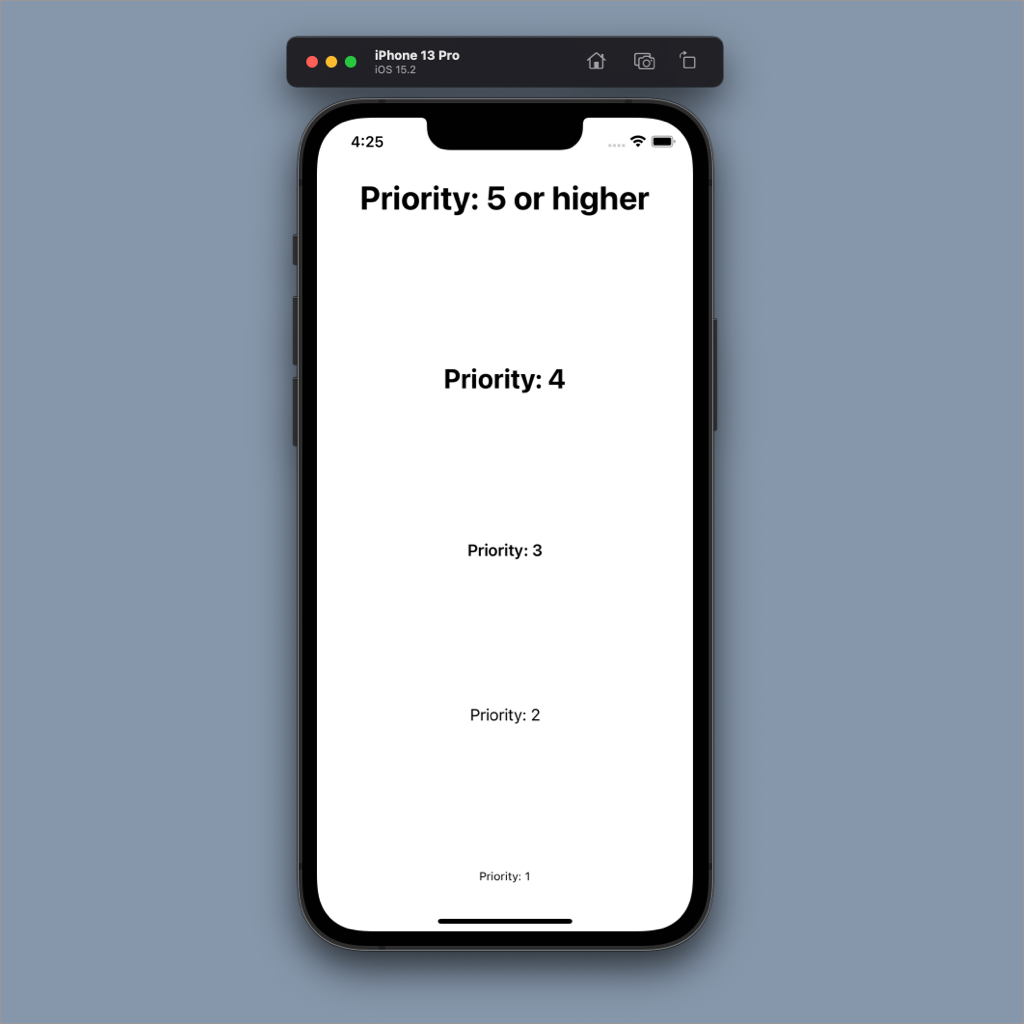
\includegraphics[width=100mm]{img/Label_priority.png}
    \end{center}
    \caption{Labelの優先度による視覚的目立たせ具合}
    \label{fig:label_priority}
  \end{minipage}
\end{figure}

\subsubsection{TextView}
図\ref{fig:TextView_priority}のように実装した.前述のLabelから文字の太さ,大きさを少し調整すると共に,最大行の指定を優先度1の場合は2行まで, 優先度2の場合は4行まで,優先度3の場合は5行まで,優先度4の場合は8行まで,優先度5以上の場合は15行を最大とした.優先度5以上でもこれ以上の大きさになることはなく,配置のみに優先度を利用する.

\begin{figure}[htbp]
  \begin{minipage}{\hsize}
    \begin{center}
       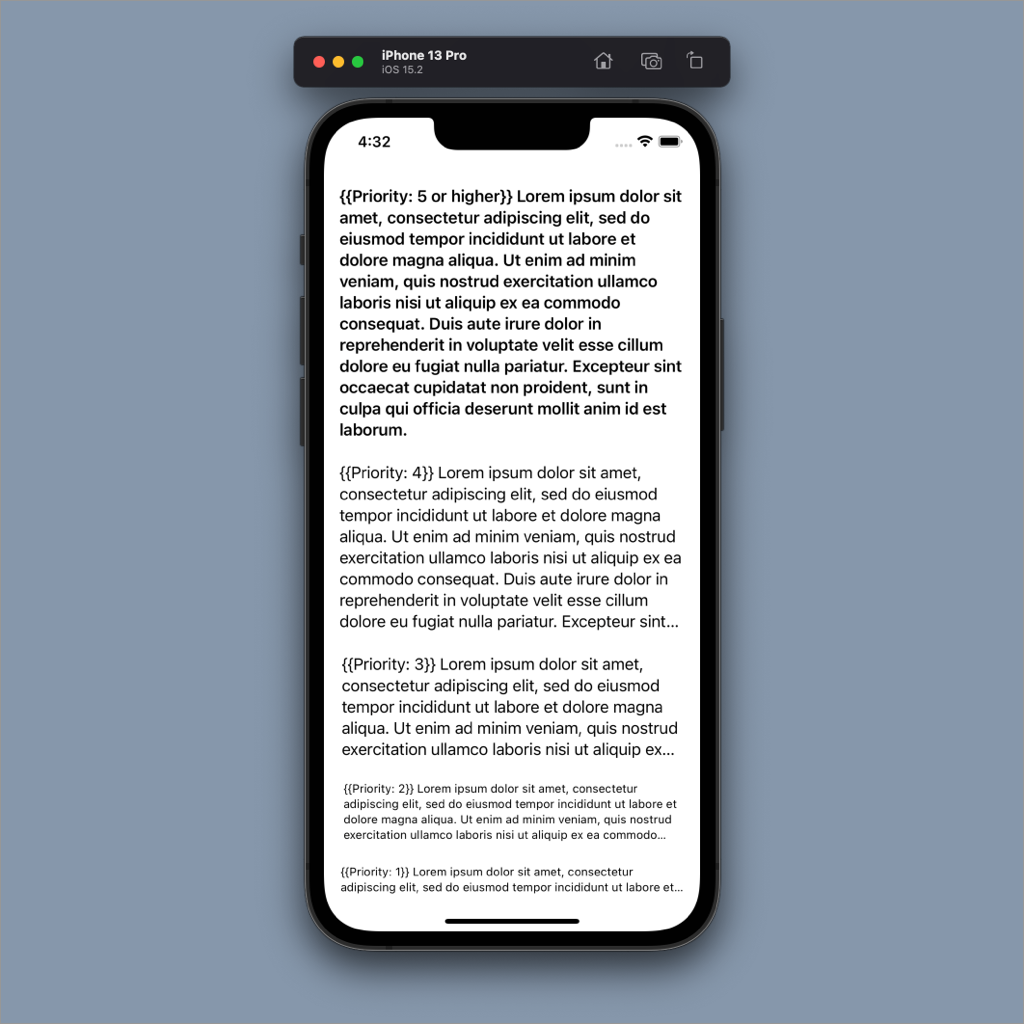
\includegraphics[width=100mm]{img/TextView_priority.png}
    \end{center}
    \caption{TextViewの優先度による視覚的目立たせ具合}
    \label{fig:TextView_priority}
  \end{minipage}
\end{figure}

\subsubsection{Button}
図\ref{fig:button_priority}のように実装した.優先度によって文字の大きさ,文字の太さ,タップエリアの大きさ,色等が変更されている.優先度5以上でもこれ以上の大きさになることはなく,配置のみに優先度を利用する.
\begin{figure}[htbp]
  \begin{minipage}{\hsize}
    \begin{center}
       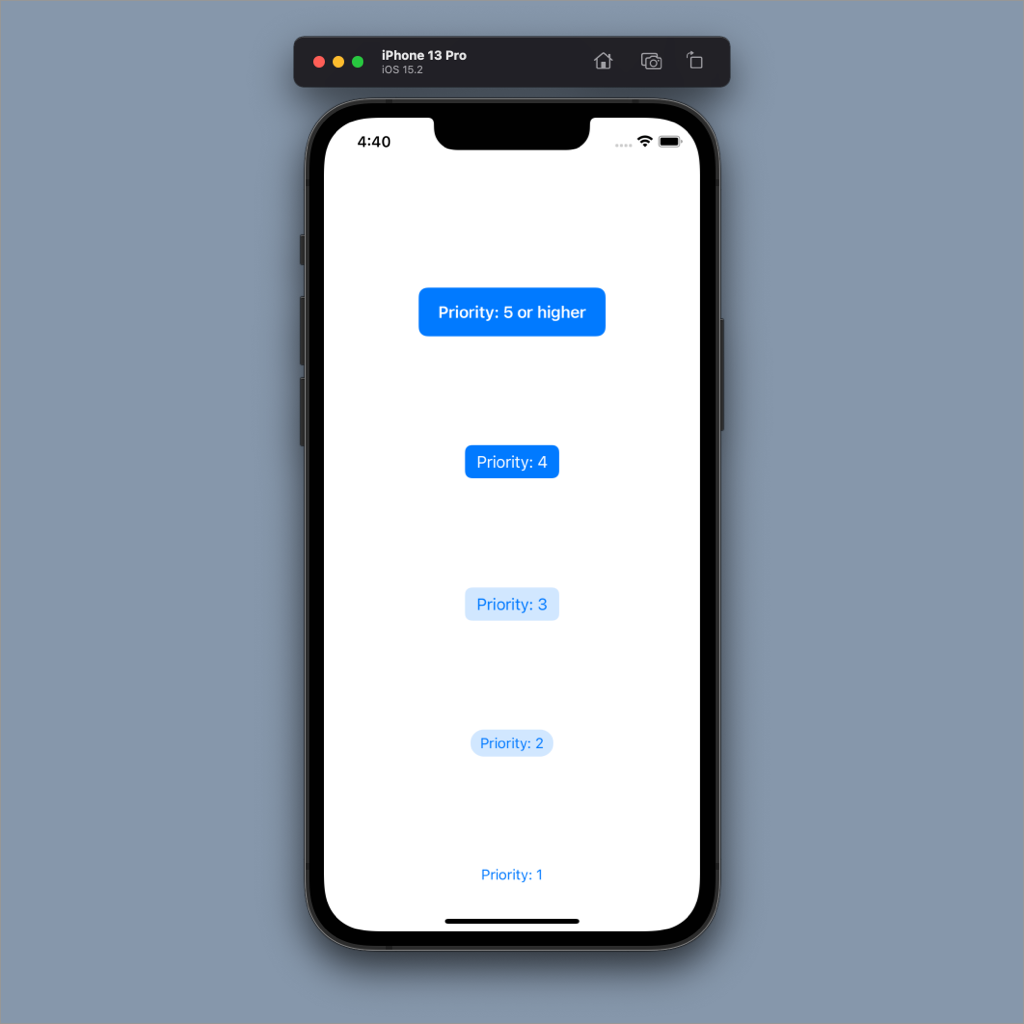
\includegraphics[width=100mm]{img/Button_priority.png}
    \end{center}
    \caption{Buttonの優先度による視覚的目立たせ具合}
    \label{fig:button_priority}
  \end{minipage}
\end{figure}

\subsubsection{Toggle}
図\ref{fig:button_priority}のように実装した.Toggleに関しては優先度で大きさや目立たせ具合が変わることはなく,優先度は配置のみに利用する.

\begin{figure}[htbp]
  \begin{minipage}{\hsize}
    \begin{center}
       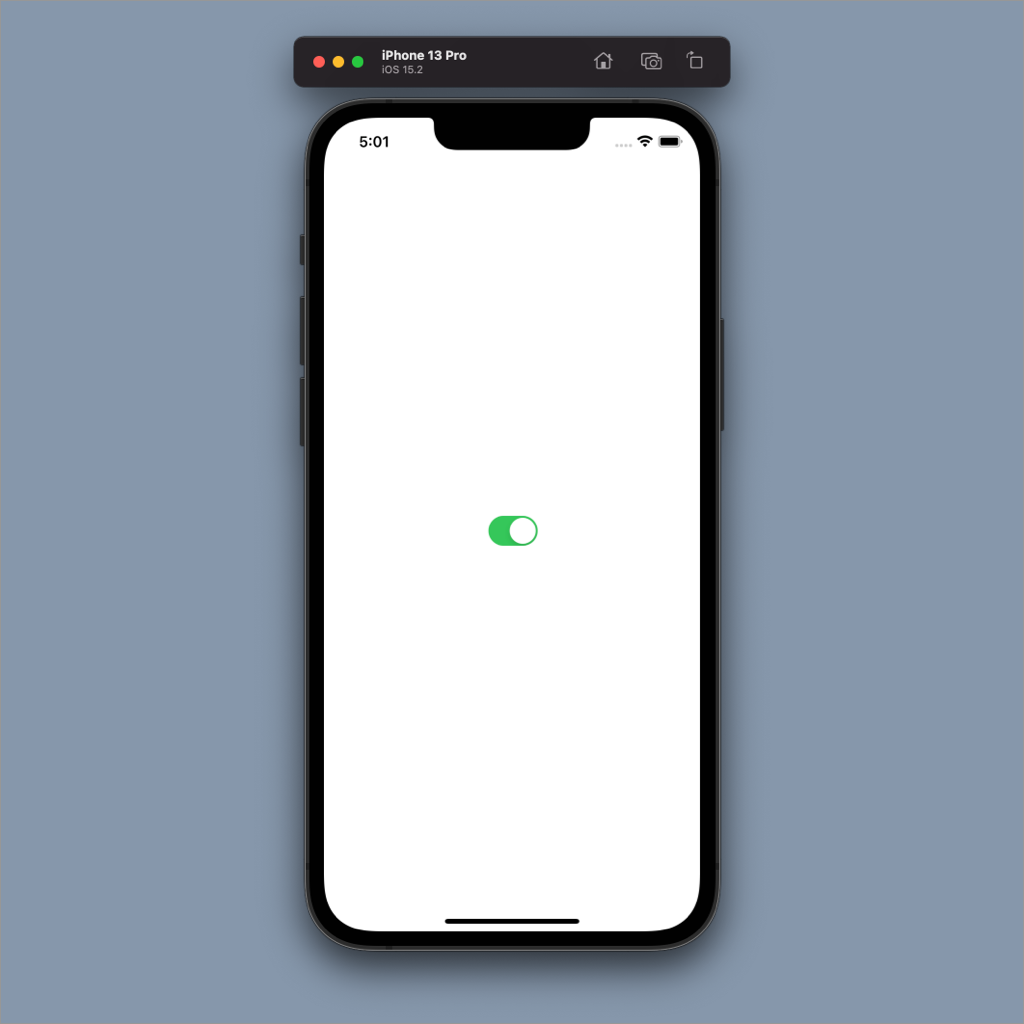
\includegraphics[width=100mm]{img/Toggle_priority.png}
    \end{center}
    \caption{Toggleの優先度による視覚的目立たせ具合}
    \label{fig:toggle_priority}
  \end{minipage}
\end{figure}

\subsubsection{Image}
図\ref{fig:image_priority}のように実装した.Imageは優先度/ 10の高さを持つ.表\ref{fig:image_priority}で使用しているサンプル画像が切れずに全てが映るようにしているため.6以上でも大きさが変化していない.

\begin{figure}[htbp]
  \begin{minipage}{\hsize}
    \begin{center}
       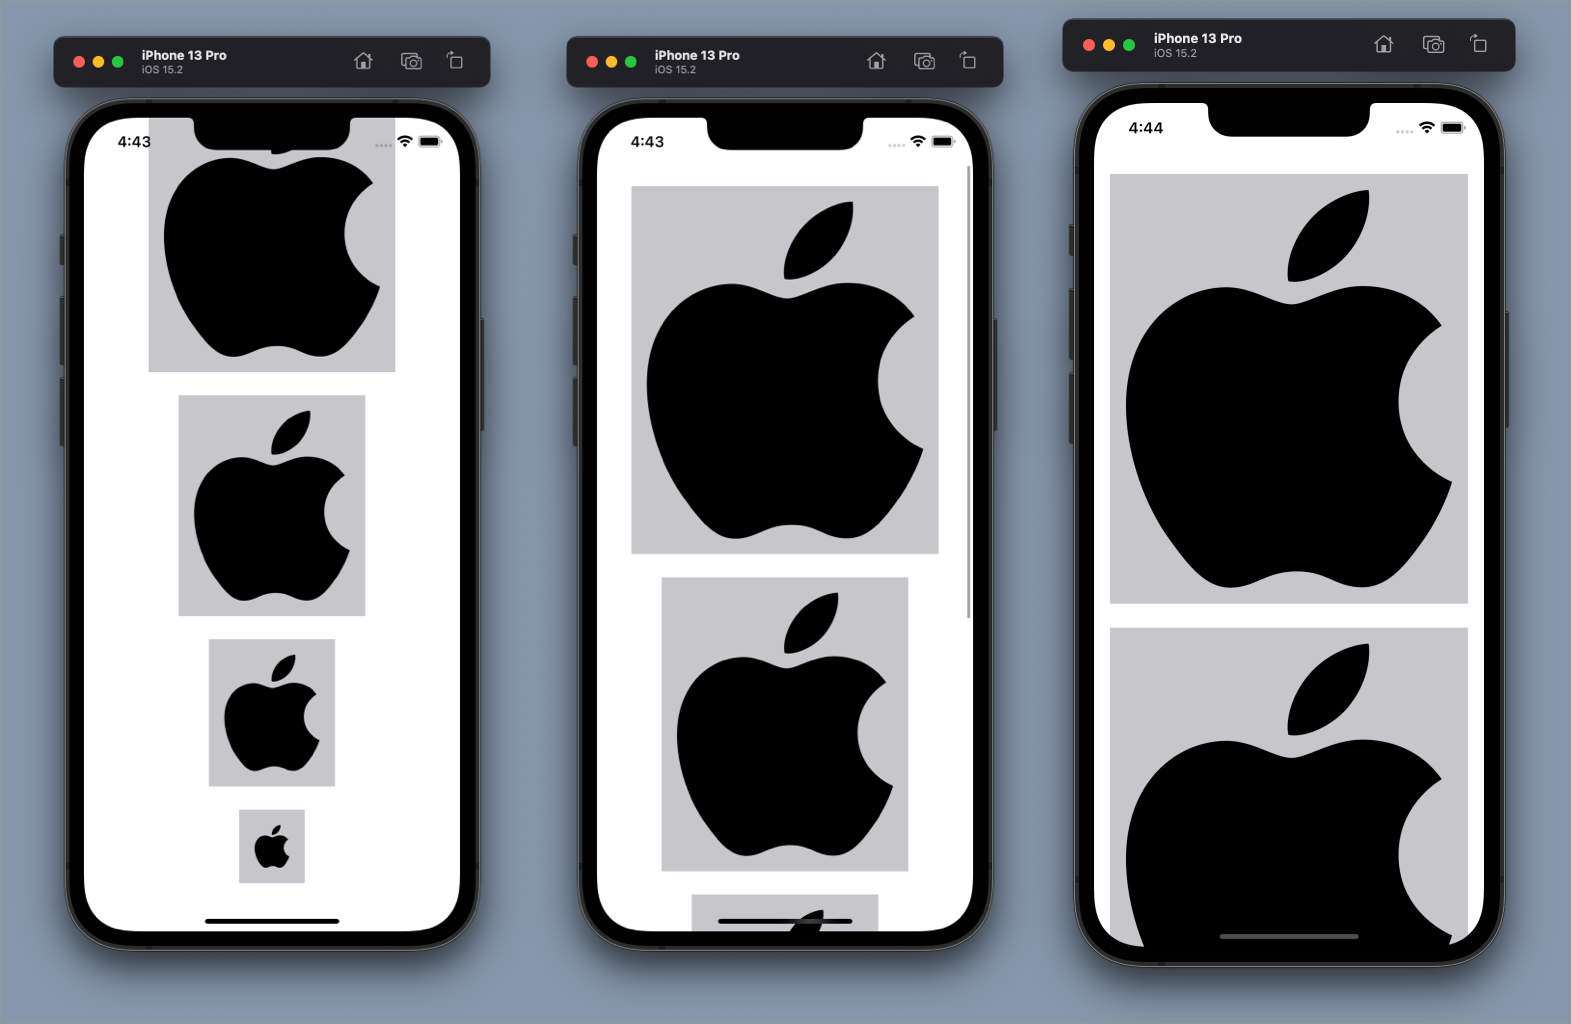
\includegraphics[width=100mm]{img/Image_priority.png}
    \end{center}
    \caption{Imageの優先度による視覚的目立たせ具合}
    \label{fig:image_priority}
  \end{minipage}
\end{figure}

\subsubsection{Map}
図\ref{fig:map_priority}のように実装した.本要素も優先度は配置のみに利用し,目立たせ具合は変化させない.また,本要素はユーザの操作を受け付けるが,特例として画面下に持ってはいかない.
\begin{figure}[htbp]
  \begin{minipage}{\hsize}
    \begin{center}
       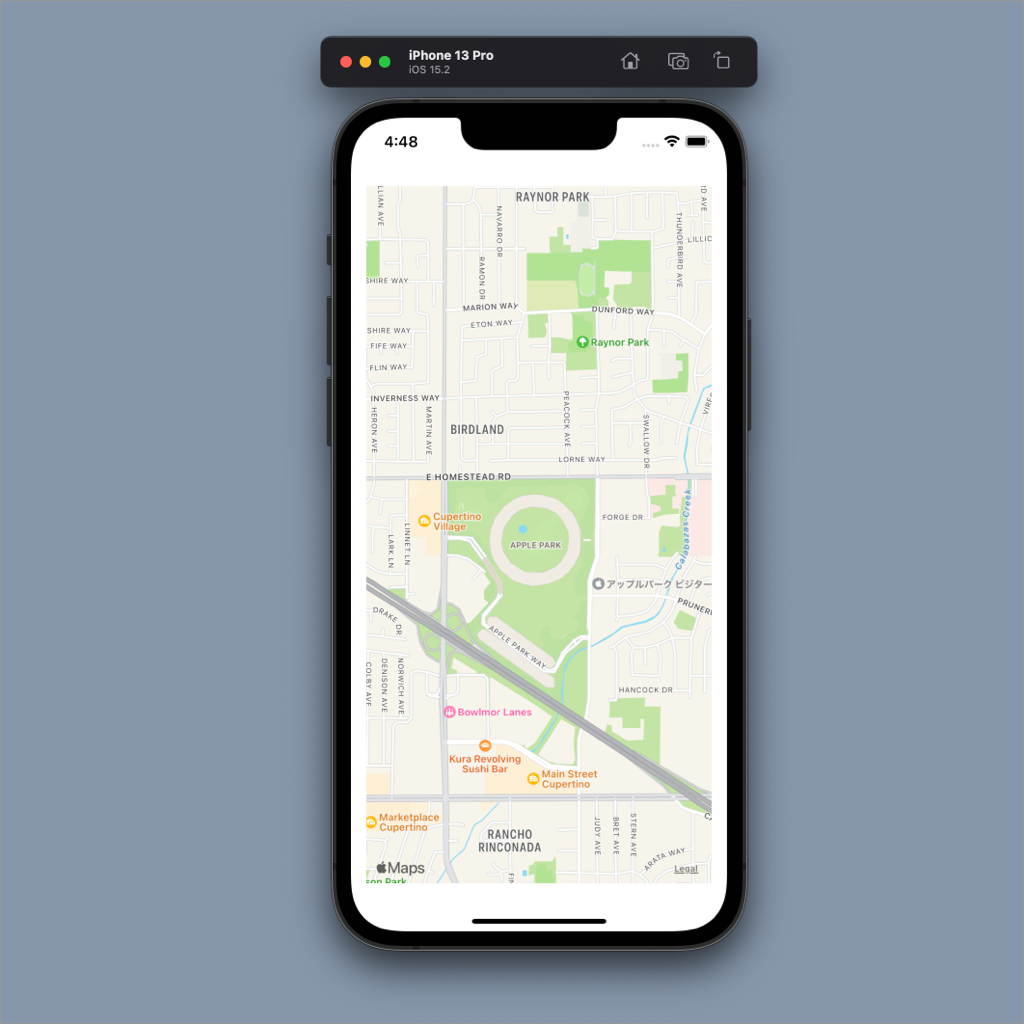
\includegraphics[width=100mm]{img/Map_priority.png}
    \end{center}
    \caption{Mapの優先度による視覚的目立たせ具合}
    \label{fig:map_priority}
  \end{minipage}
\end{figure}

\subsubsection{DatePicker}
図\ref{fig:datepicker_priority}のように実装した.優先度1,2では画面右下のコンパクトスタイル,優先度3ではドラムロールスタイル,4以上ではカレンダースタイルで日付を選ぶようにした.でもこれ以上の大きさになることはなく,余白として扱われる.

\begin{figure}[htbp]
  \begin{minipage}{\hsize}
    \begin{center}
       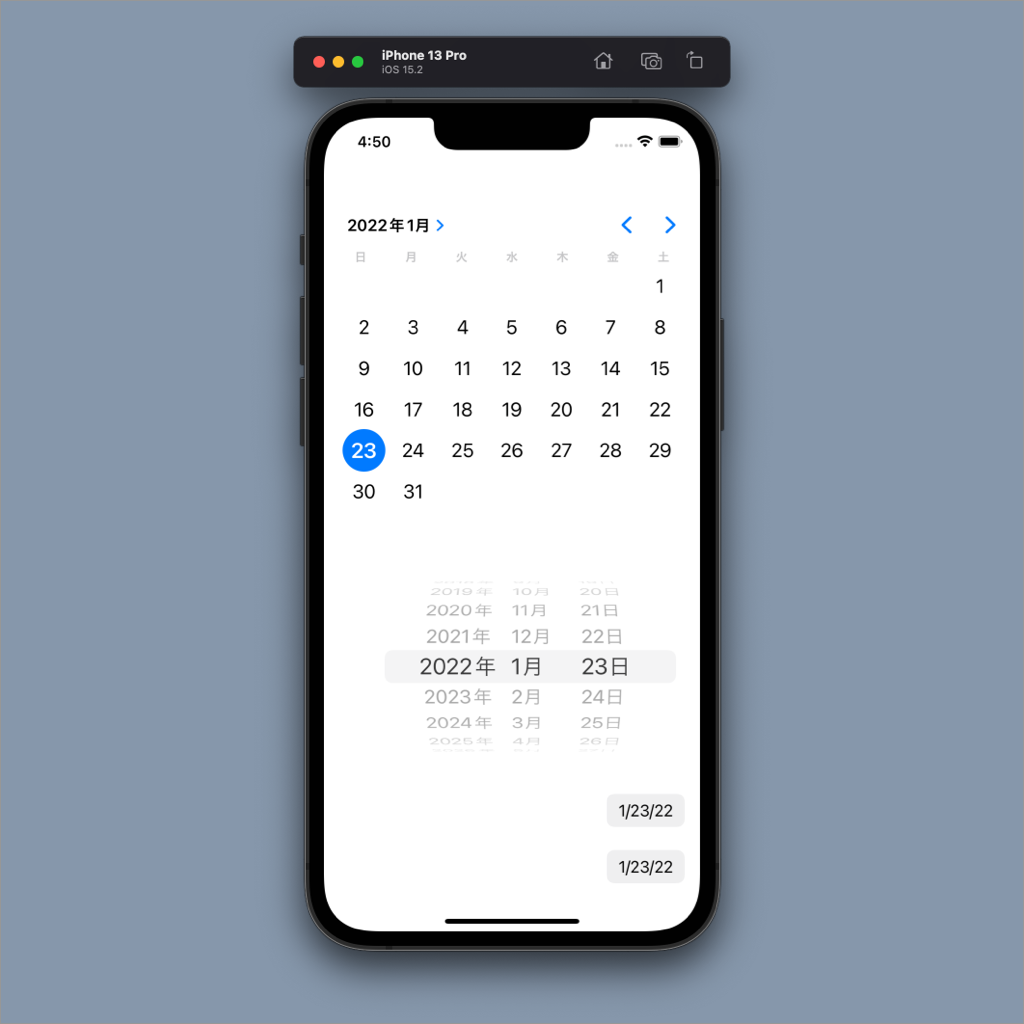
\includegraphics[width=100mm]{img/DatePicker_priority.png}
    \end{center}
    \caption{DatePickerの優先度による視覚的目立たせ具合}
    \label{fig:datepicker_priority}
  \end{minipage}
\end{figure}

\subsubsection{Slider}
図\ref{fig:slider_priority}のように実装した.優先度による見た目の変化はなく,配置のみに利用される.

\begin{figure}[htbp]
  \begin{minipage}{\hsize}
    \begin{center}
       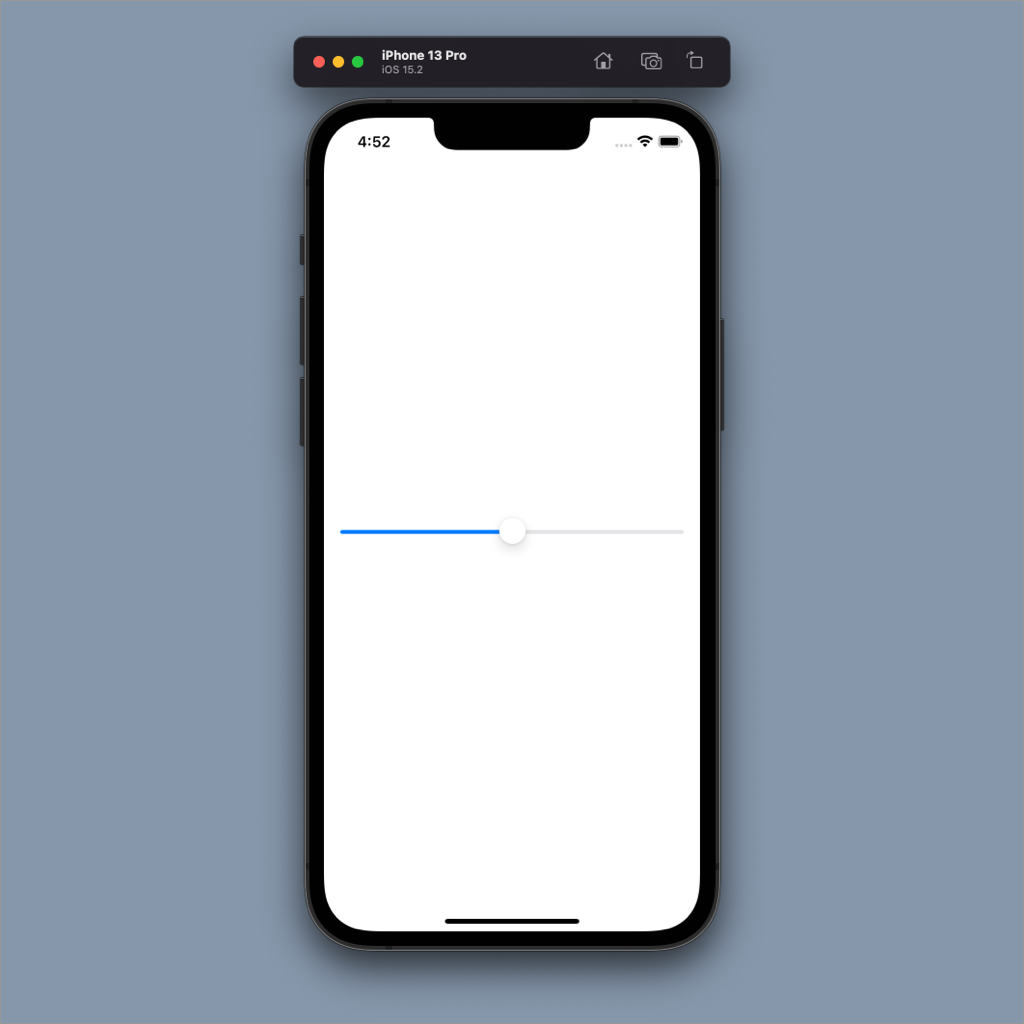
\includegraphics[width=100mm]{img/Slider_priority.png}
    \end{center}
    \caption{Sliderの優先度による視覚的目立たせ具合}
    \label{fig:slider_priority}
  \end{minipage}
\end{figure}


\subsection{グルーピング}
グルーピングでは前述の要素をグループに入れて表示する.グループ内の要素の優先度から自己の優先度を決定する実装にした.
グループの表示は基本的にはroot Group(自分が他のグループの中の要素ではないグループ)が横方向に配置している.しかしながらそこには横方向には適さないUIの場合もあるので縦方向に指定するオプションも用意した.
\subsubsection{グルーピングの入れ子構造}
グルーピングの入れ子構造では親グループの方向が縦ならば横,横なら縦と,縦方向の配置と横方向の表示を交互で表示するように実装した.前述同様,強制的にグループの方向を決めることもできる.

\section{システムの有効性についての実験}

\subsection{既存UIの再現}
前セクションでは本システムの表示アルゴリズムの具体的なシステムの実装を説明した.本セクションでは既存UIを要素,優先度,グルーピングに落とし込み,本システムを利用して再度UI構築を行う実験をおこなった.
本実験ではSNSフィード画面(Instagram), ログイン画面(NIKKEI Wave),リスト画面(設定),地図画面(Maps)についておこなった.
\subsubsection{SNSフィード画面(Instagram)}
図\ref{fig:instagram_screenshot}を解析し, 図\ref{fig:instagram_ViewStructure}の要素,優先度グルーピングを得ることができた.図\ref{fig:instagram_ViewStructure}の構造を複数個本システムにインプットしたところ図\ref{fig:instagram_autogen}を得ることができた.


\begin{figure}[htbp]
  \begin{minipage}{\hsize}
    \begin{center}
       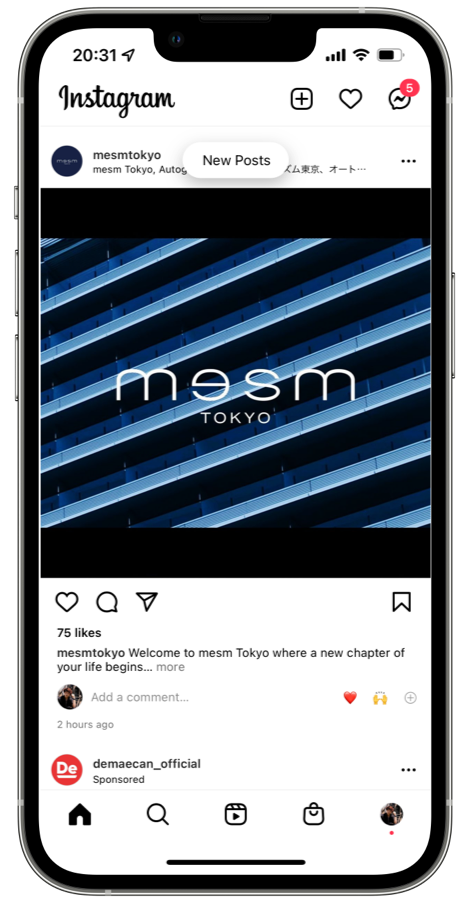
\includegraphics[width=50mm]{img/instagram_screenshot.png}
    \end{center}
    \caption{既存のSNSフィード画面(Instagram)}
    \label{fig:instagram_screenshot}
  \end{minipage}
\end{figure}

\begin{figure}[htbp]
  \begin{minipage}{\hsize}
    \begin{center}
       
\includegraphics[width=100mm]{img/Instagram_ViewStructure.png}
    \end{center}
    \caption{既存のSNSフィード画面(Instagram)の要素,優先度,グルーピング}
    \label{fig:instagram_ViewStructure}
  \end{minipage}
\end{figure}

\begin{figure}[htbp]
  \begin{minipage}{\hsize}
    \begin{center}
       \includegraphics[width=50mm]{img/Instagram_autogen.png}
    \end{center}
    \caption{本システムで再構築されたSNSフィード画面}
    \label{fig:instagram_autogen}
  \end{minipage}
\end{figure}

\subsubsection{ログイン画面(NIKKEI Wave)}
図\ref{fig:wave_screenshot}を解析し, 図\ref{fig:wave_ViewStructure}の要素,優先度グルーピングを得ることができた.図\ref{fig:wave_ViewStructure}の構造を複数個本システムにインプットしたところ図\ref{fig:wave_autogen}を得ることができた.

\begin{figure}[htbp]
  \begin{minipage}{\hsize}
    \begin{center}
       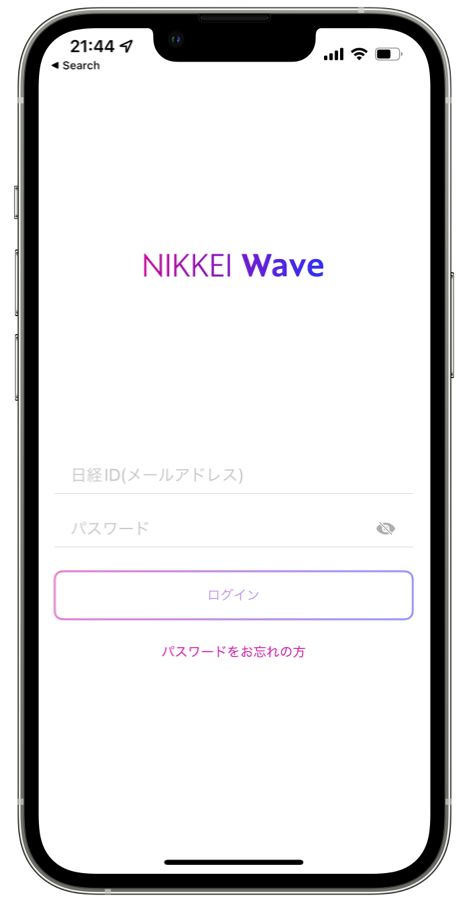
\includegraphics[width=50mm]{img/wave_screenshot.png}
    \end{center}
    \caption{既存のログイン画面(NIKKEI Wave)}
    \label{fig:wave_screenshot}
  \end{minipage}
\end{figure}

\begin{figure}[htbp]
  \begin{minipage}{\hsize}
    \begin{center}
       \includegraphics[width=100mm]{img/wave_ViewStructure.png}
    \end{center}
    \caption{既存のログイン画面(NIKKEI Wave)の要素,優先度,グルーピング}
    \label{fig:wave_ViewStructure}
  \end{minipage}
\end{figure}

\begin{figure}[htbp]
  \begin{minipage}{\hsize}
    \begin{center}
       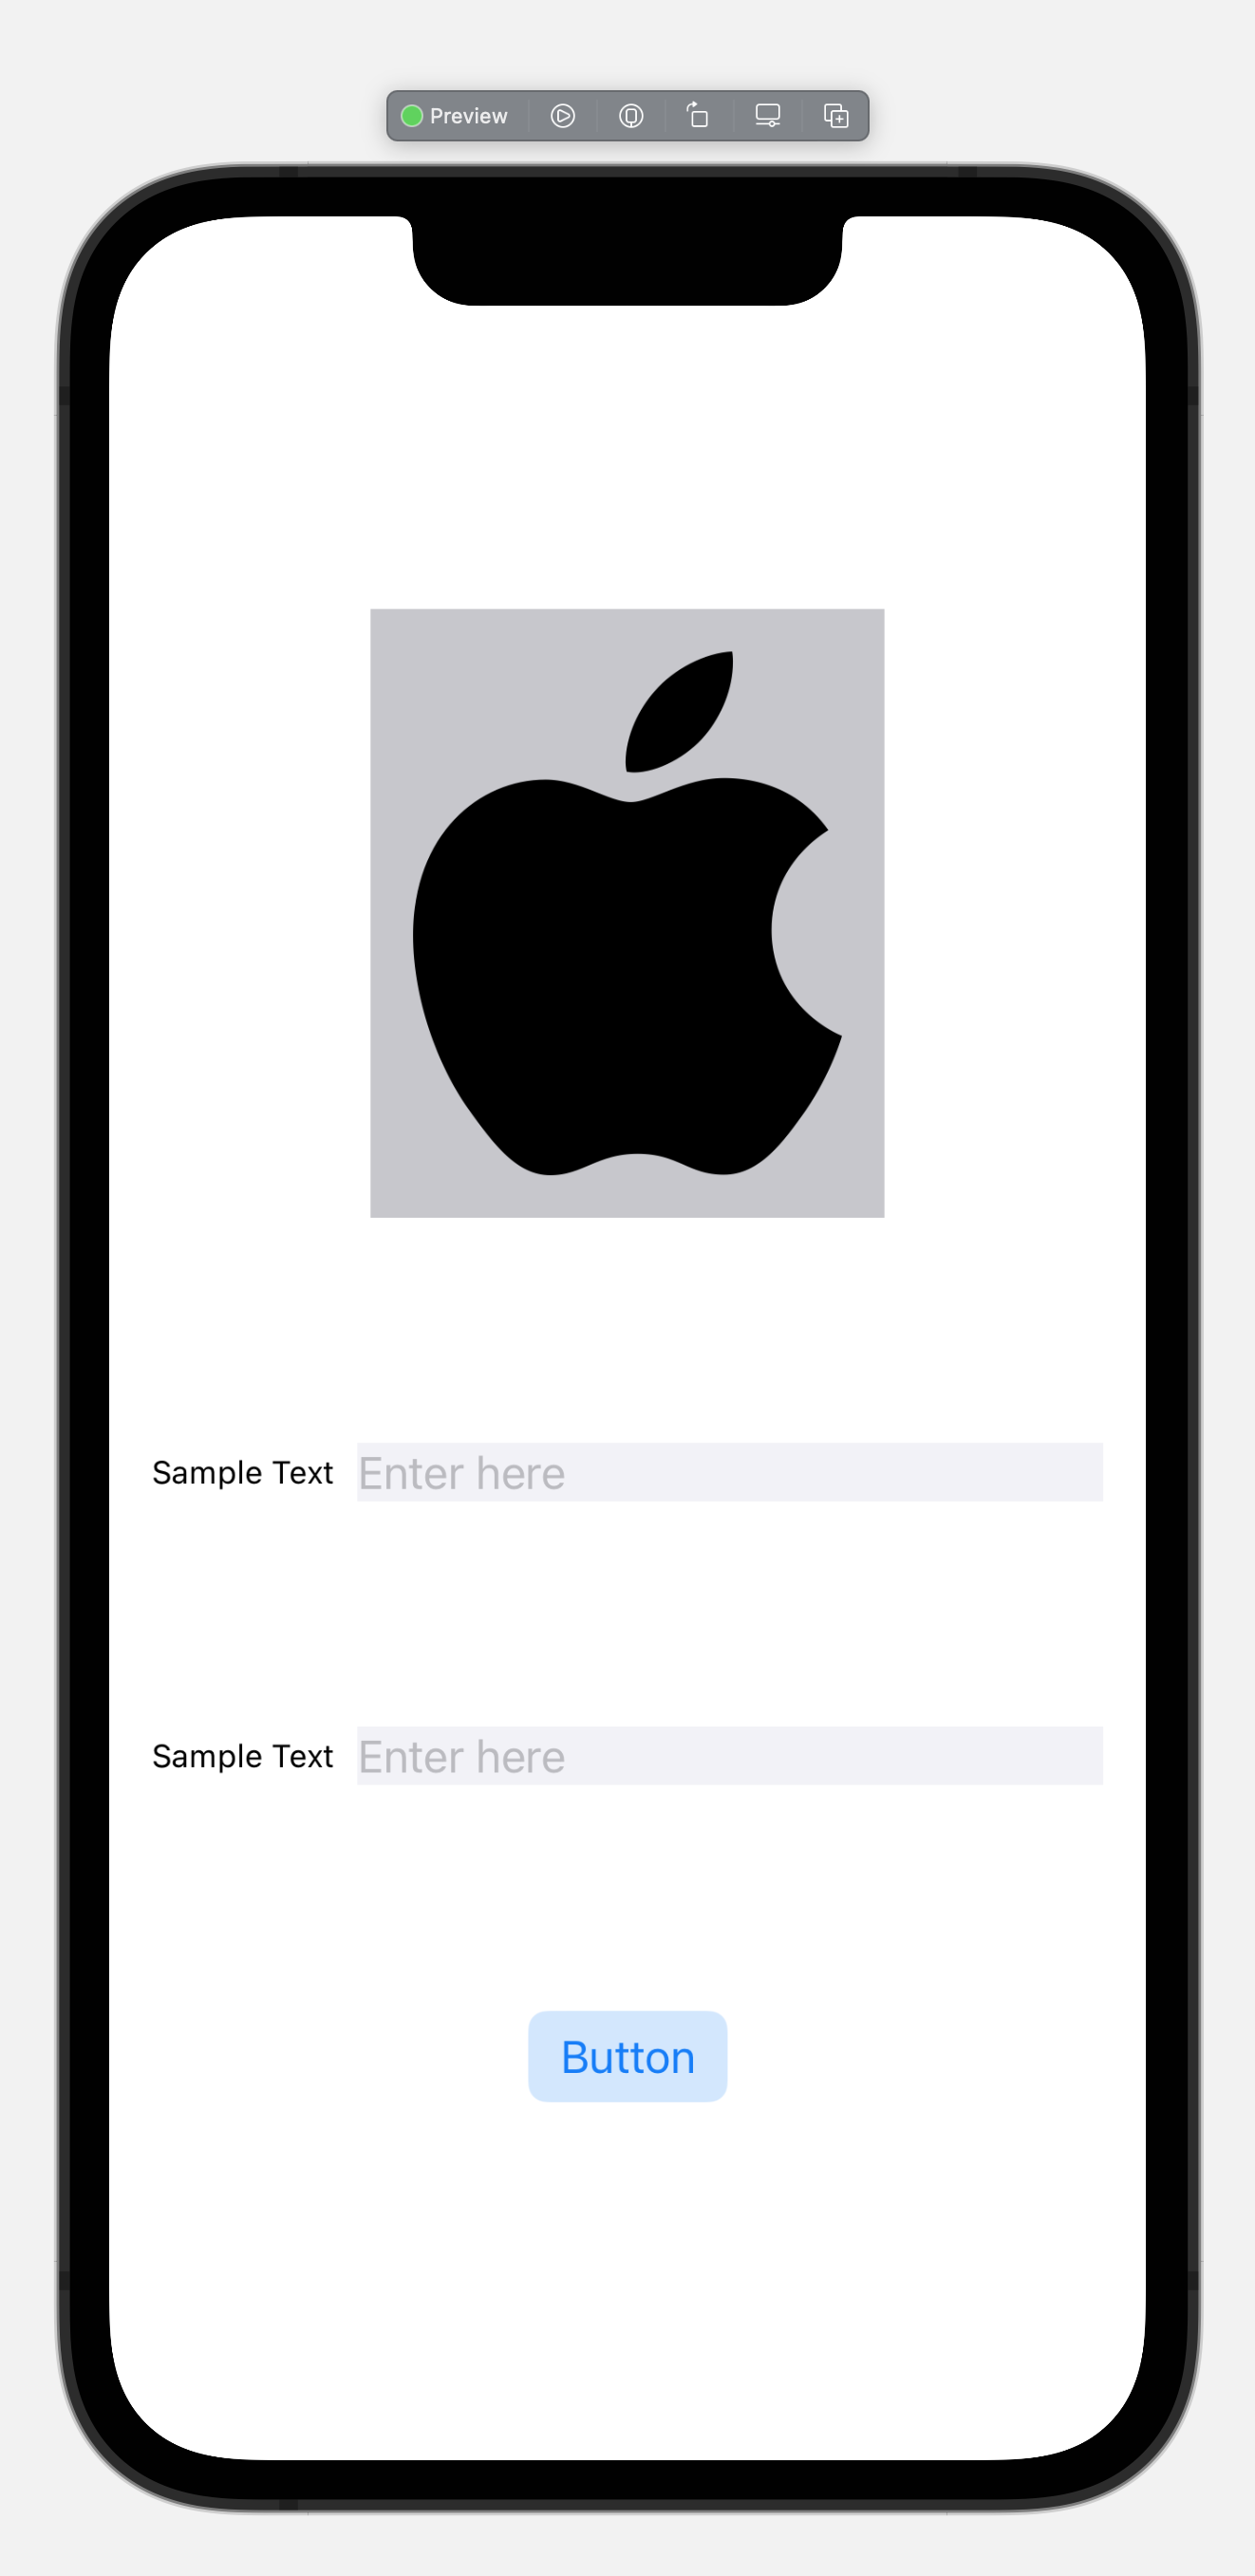
\includegraphics[width=50mm]{img/wave_autogen.png}
    \end{center}
    \caption{本システムで再構築されたログイン画面}
    \label{fig:wave_autogen}
  \end{minipage}
\end{figure}

\subsubsection{リスト画面(設定)}
図\ref{fig:Settings_screenshot}を解析し, 図\ref{fig:Settings_ViewStructure}の要素,優先度グルーピングを得ることができた.図\ref{fig:Settings_ViewStructure}の構造を複数個本システムにインプットしたところ図\ref{fig:Settings_autogen}を得ることができた.

\begin{figure}[htbp]
  \begin{minipage}{\hsize}
    \begin{center}
       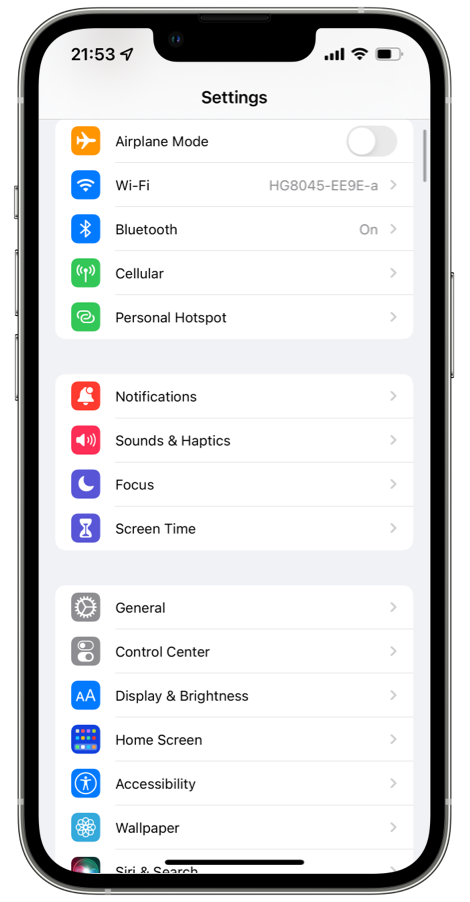
\includegraphics[width=50mm]{img/Settings_screenshot.png}
    \end{center}
    \caption{リスト画面(Settings)}
    \label{fig:Settings_screenshot}
  \end{minipage}
\end{figure}

\begin{figure}[htbp]
  \begin{minipage}{\hsize}
    \begin{center}
       
\includegraphics[width=30mm]{img/Settings_ViewStructure.png}
    \end{center}
    \caption{リスト画面(Settings)の要素,優先度,グルーピング}
    \label{fig:Settings_ViewStructure}
  \end{minipage}
\end{figure}

\begin{figure}[htbp]
  \begin{minipage}{\hsize}
    \begin{center}
       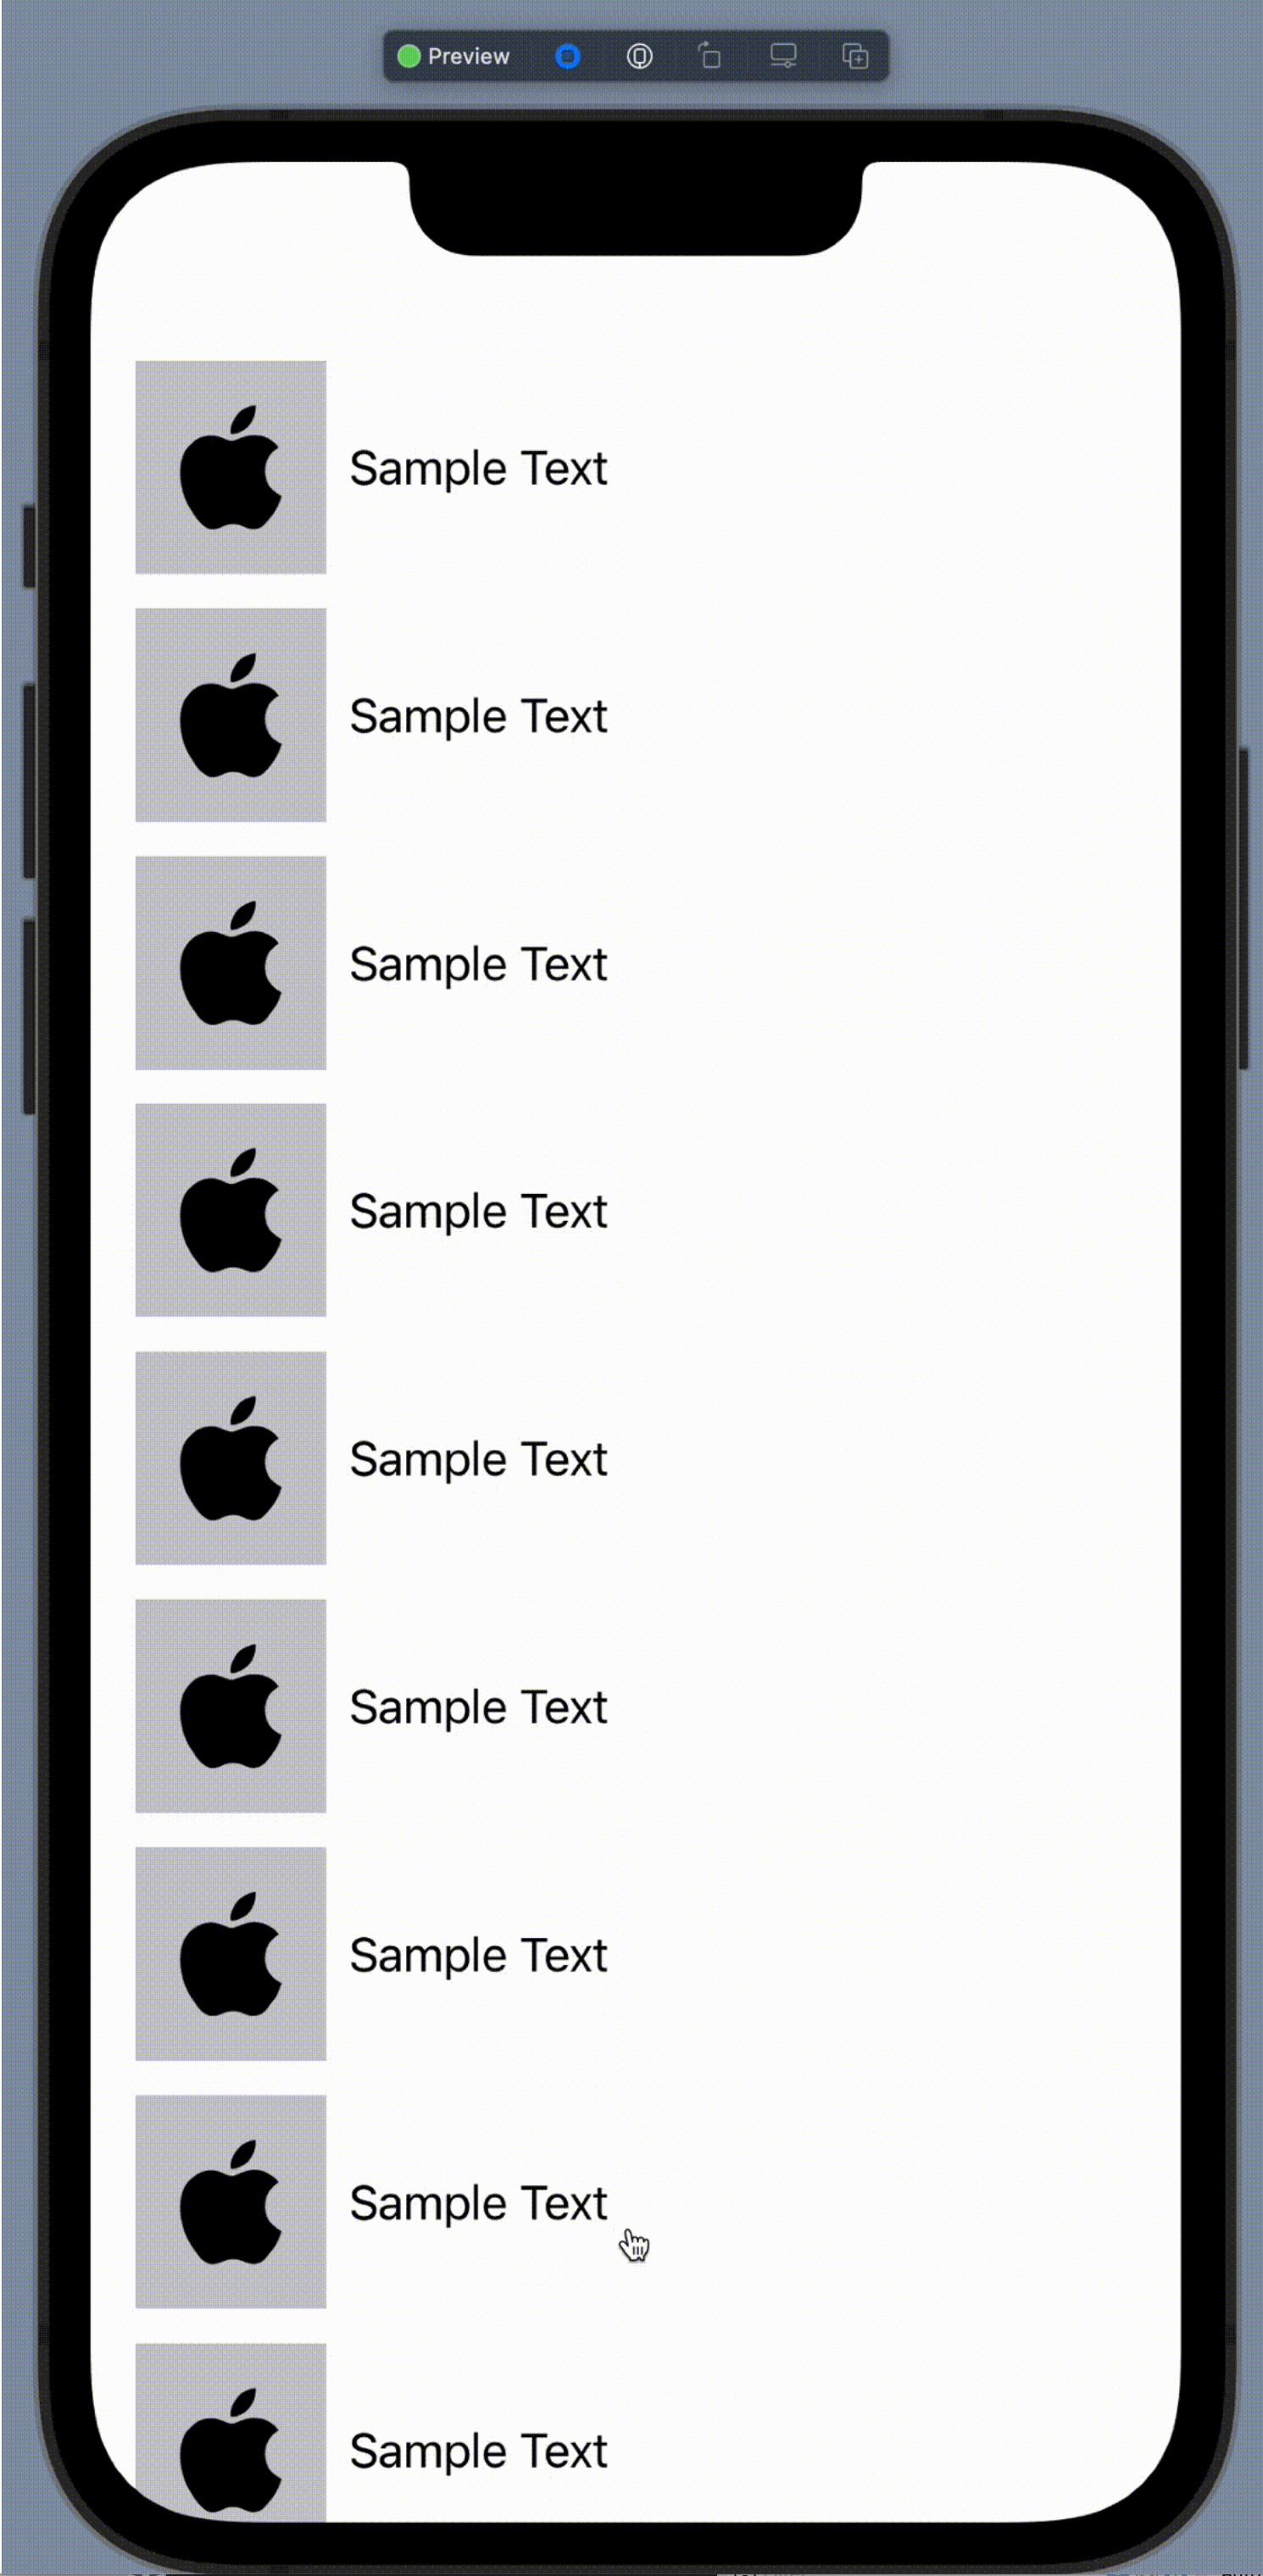
\includegraphics[width=50mm]{img/Settings_autogen.png}
    \end{center}
    \caption{リスト画面}
    \label{fig:Settings_autogen}
  \end{minipage}
\end{figure}


\subsubsection{地図画面(Maps)}
図\ref{fig:Maps_screenshot}を解析し, 図\ref{fig:Maps_ViewStructure}の要素,優先度グルーピングを得ることができた.図\ref{fig:Maps_ViewStructure}の構造を複数個本システムにインプットしたところ図\ref{fig:Maps_autogen}を得ることができた.


\begin{figure}[htbp]
  \begin{minipage}{\hsize}
    \begin{center}
       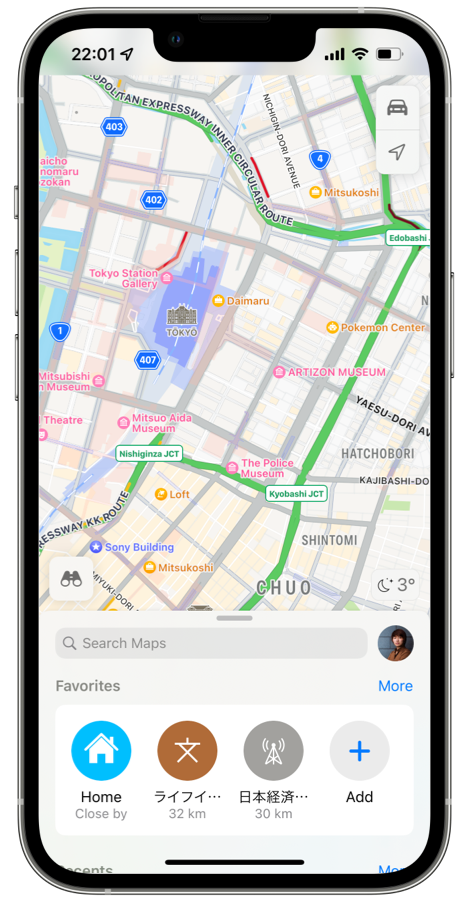
\includegraphics[width=50mm]{img/Maps_screenshot.png}
    \end{center}
    \caption{地図画面(Maps)}
    \label{fig:Maps_screenshot}
  \end{minipage}
\end{figure}

\begin{figure}[htbp]
  \begin{minipage}{\hsize}
    \begin{center}
       
\includegraphics[width=100mm]{img/Maps_ViewStructure.png}
    \end{center}
    \caption{地図画面(Maps)の要素,優先度,グルーピング}
    \label{fig:Maps_ViewStructure}
  \end{minipage}
\end{figure}

\begin{figure}[htbp]
  \begin{minipage}{\hsize}
    \begin{center}
       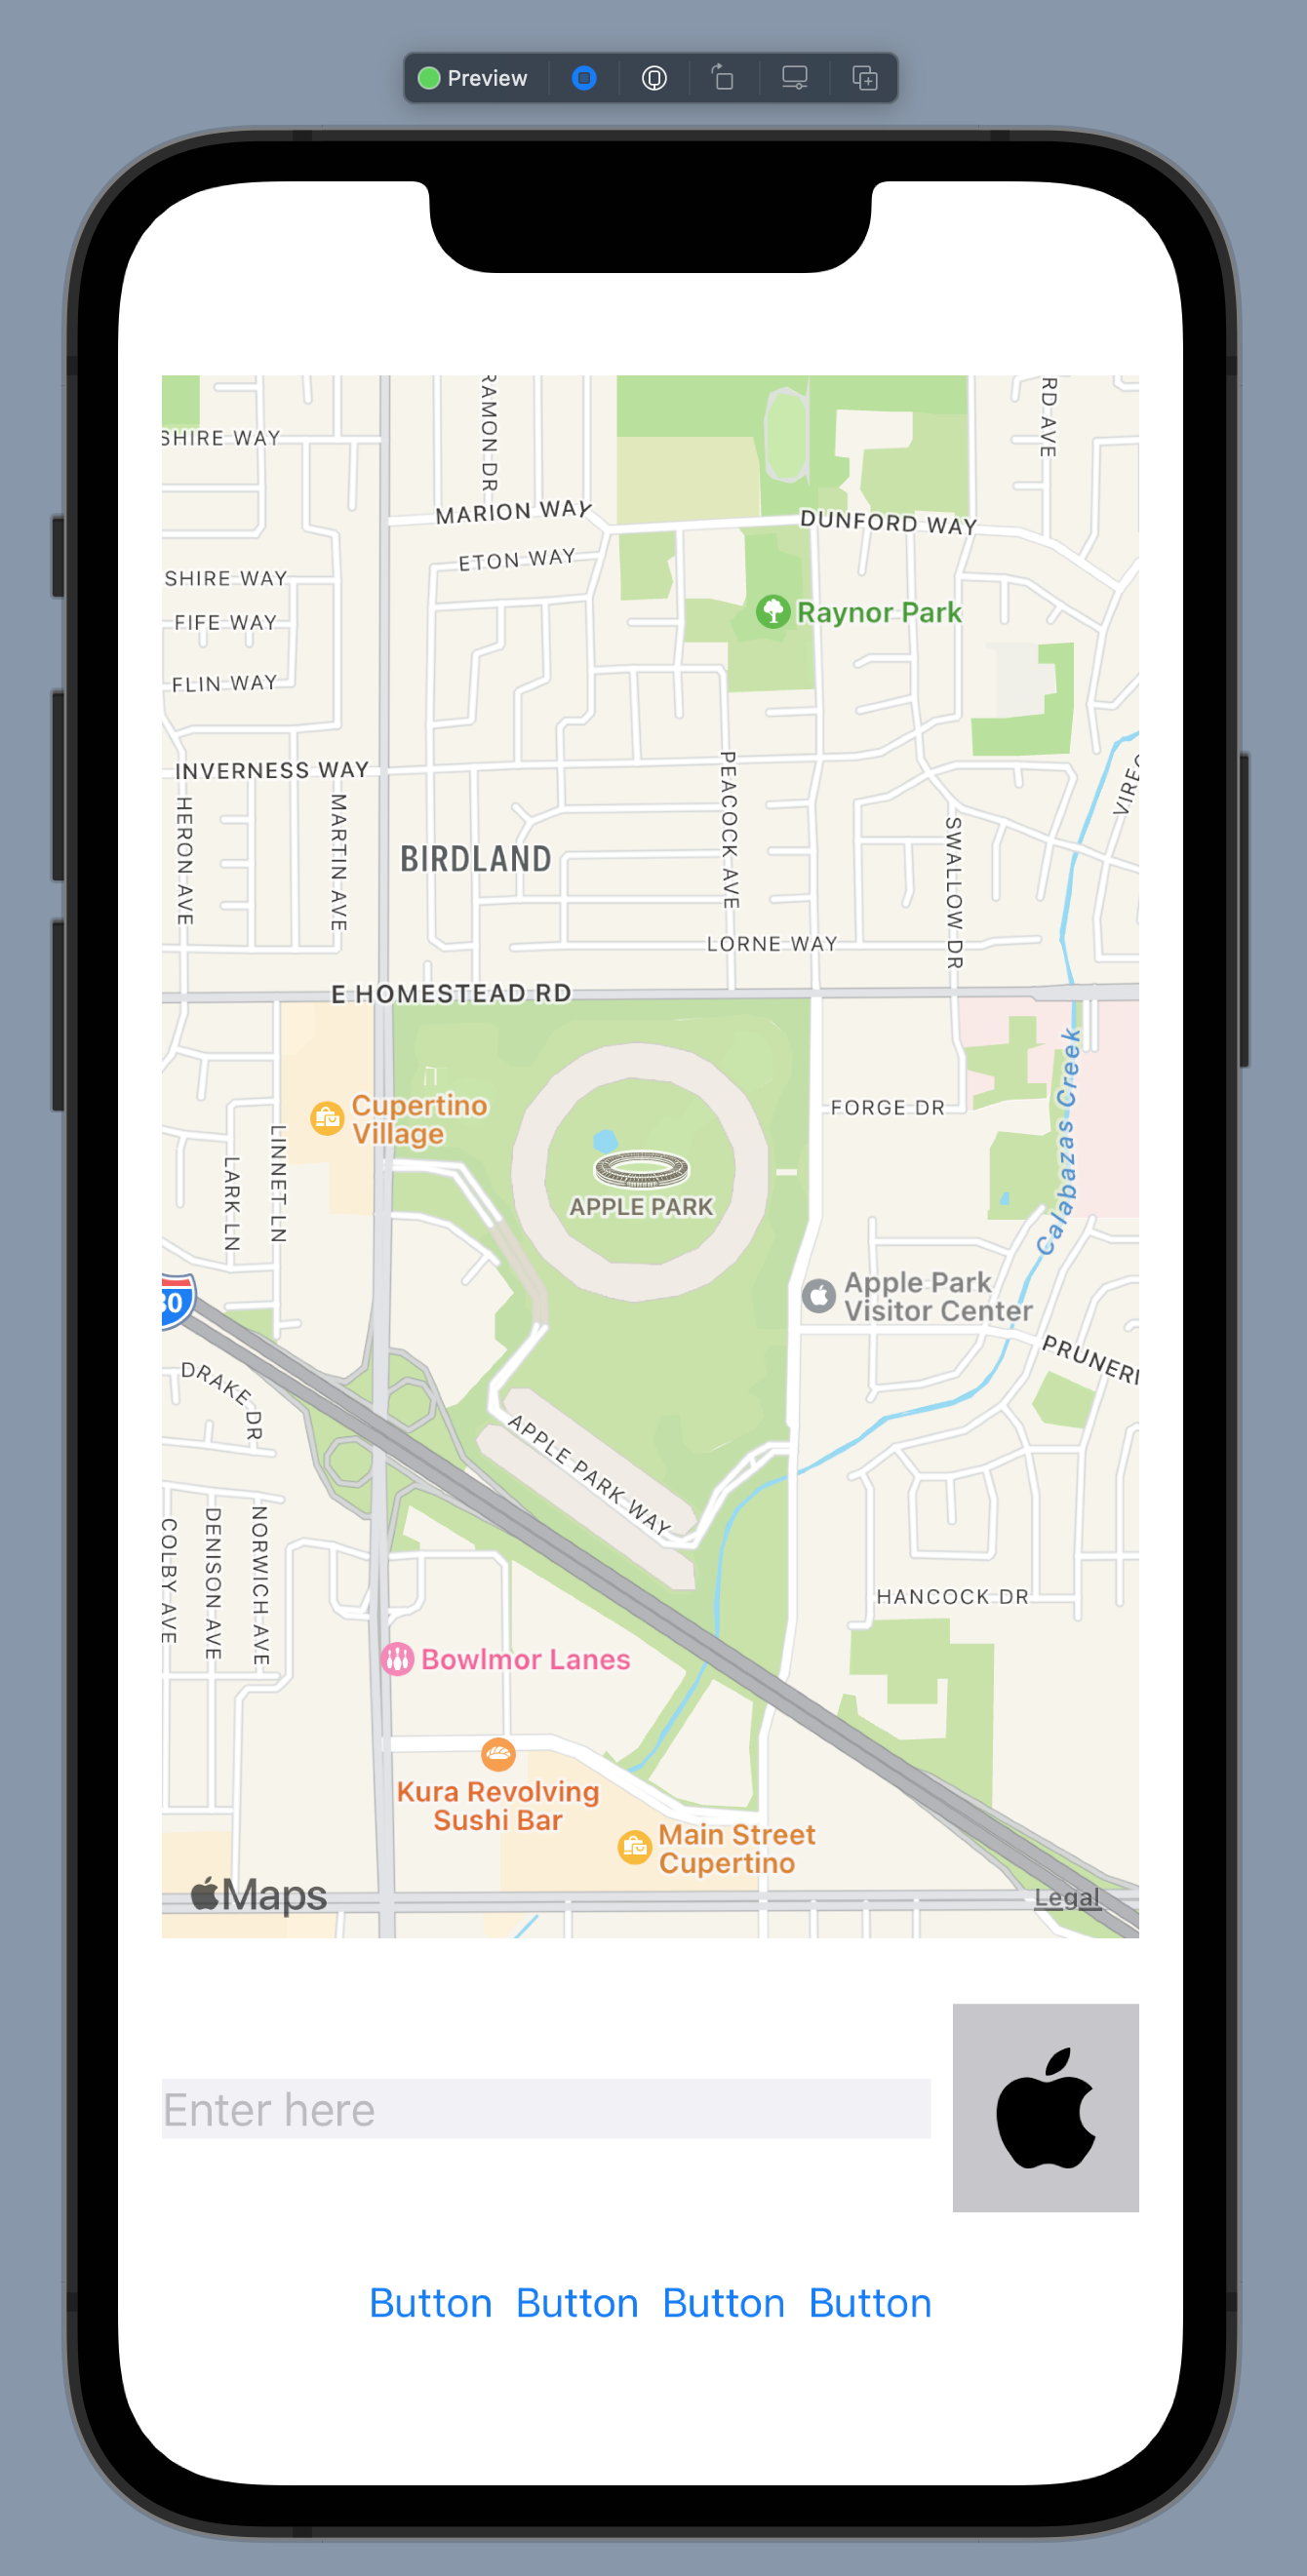
\includegraphics[width=50mm]{img/Maps_autogen.png}
    \end{center}
    \caption{地図画面}
    \label{fig:Maps_autogen}
  \end{minipage}
\end{figure}


\subsection{ユーザテスト}
普段からiOSネイティブアプリケーションの企画,設計,開発を行う14-17歳の中高生男女を対象に設計段階のアプリにおいて本システムを利用しUIの自動生成の有用性を測る実験とアンケートを実施した.
本ユーザテストでは従来のUIデザイン手法ではなく,画面内の要素,優先度,グルーピングを抽出することの難易度調査,期待するUIが自動生成されるかどうか,また優先度を編集することでの本システムとのインタラクションによるUI設計があるかを調査した.
\subsection{対象と手続き}
本ユーザテストではコンピュータの基本操作は理解しており,日頃からiOSネイティブアプリケーションの企画,設計,開発をおこなっている中高生を対象とした.

被験者には事前説明として画面内の要素,優先度,グルーピングで構成できる旨の説明を行い,使用できる要素の種類一覧(表\ref{table:ui_elements})を示した.

実験では白紙一枚を渡し,白紙に図\ref{fig:instagram_ViewStructure},図\ref{fig:wave_ViewStructure},図\ref{fig:Settings_ViewStructure},図\ref{fig:Maps_ViewStructure},にならった 要素,優先度,グルーピングの図示を行わせ,自動生成システムにかけ実際にUIを出力させた.


\begin{figure}[htbp]
  \begin{minipage}{\hsize}
    \begin{center}
       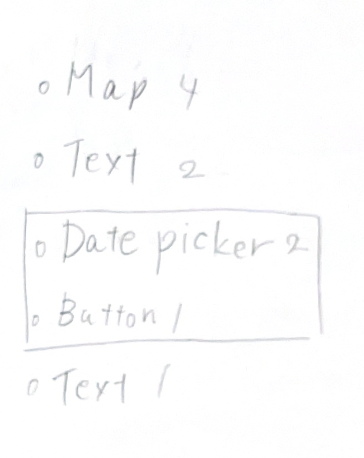
\includegraphics[width=50mm]{img/usertest_viewstructure_1.png}
    \end{center}
    \caption{被験者A記入用紙}
    \label{fig:usertest_viewstructure_1}
  \end{minipage}
\end{figure}

\begin{figure}[htbp]
  \begin{minipage}{\hsize}
    \begin{center}
       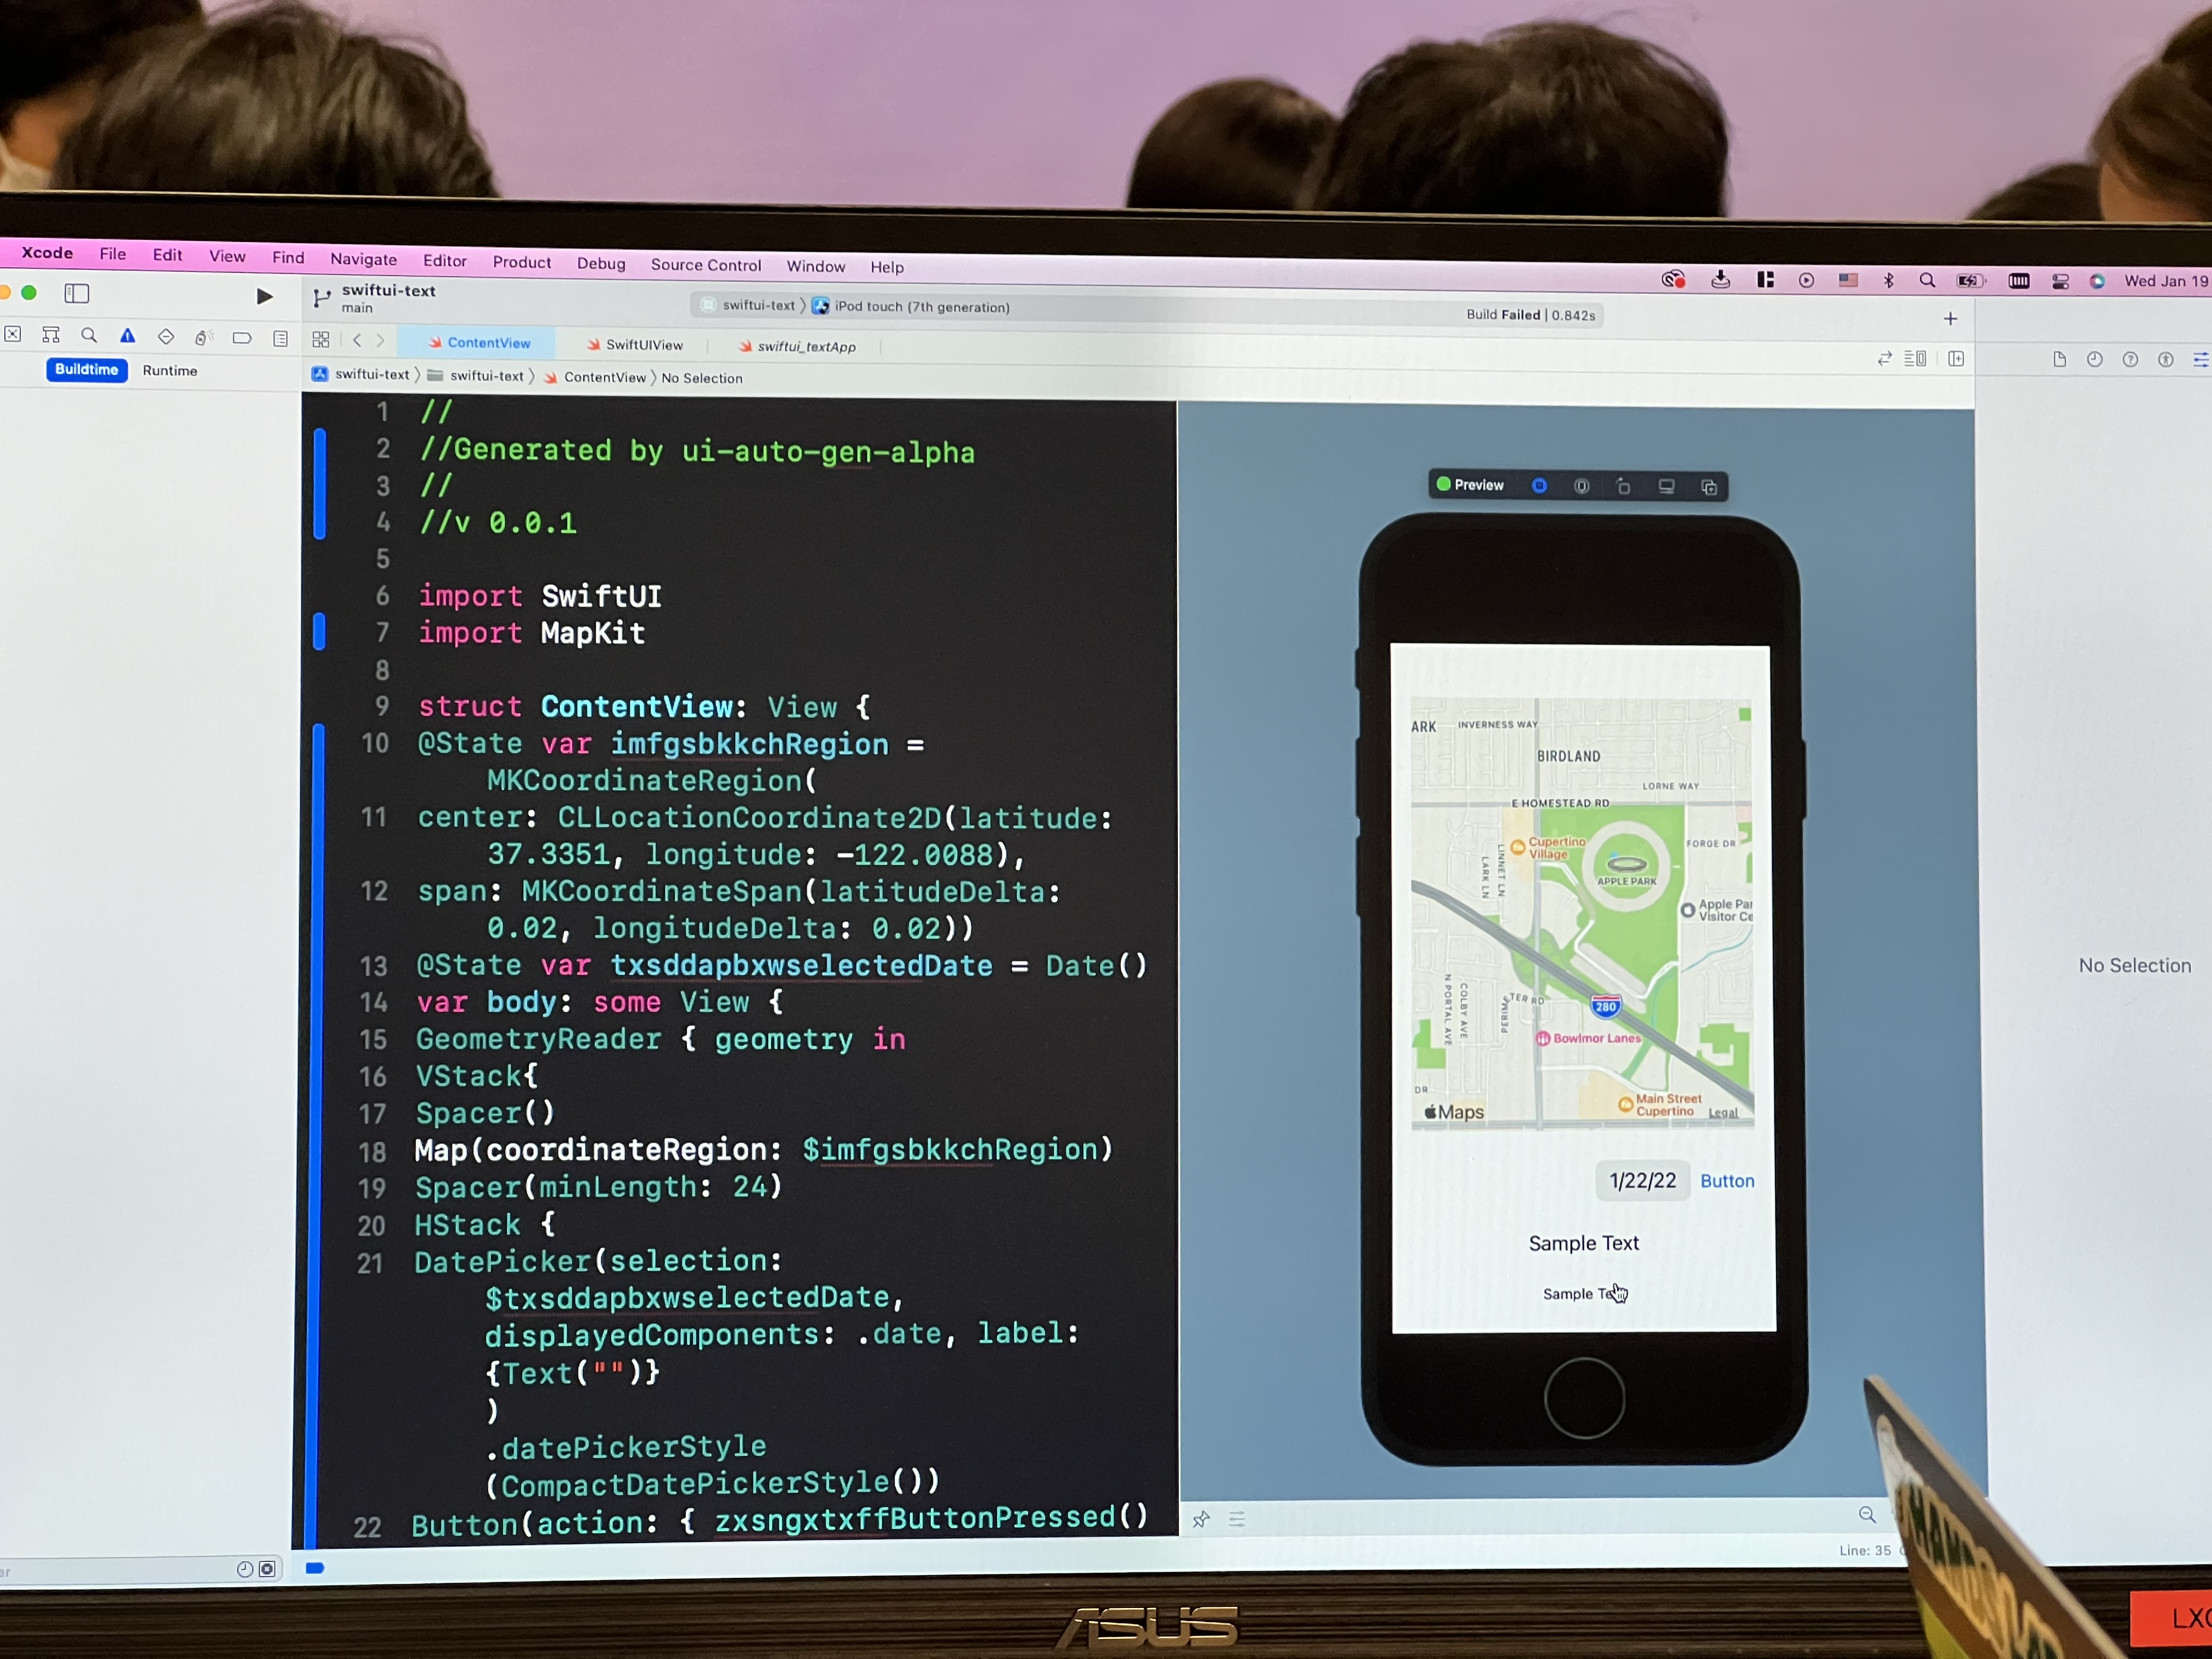
\includegraphics[width=100mm]{img/usertest_autogen_1.jpeg}
    \end{center}
    \caption{被験者A自動生成UI}
    \label{fig:usertest_autogen_1}
  \end{minipage}
\end{figure}



\begin{figure}[htbp]
  \begin{minipage}{\hsize}
    \begin{center}
       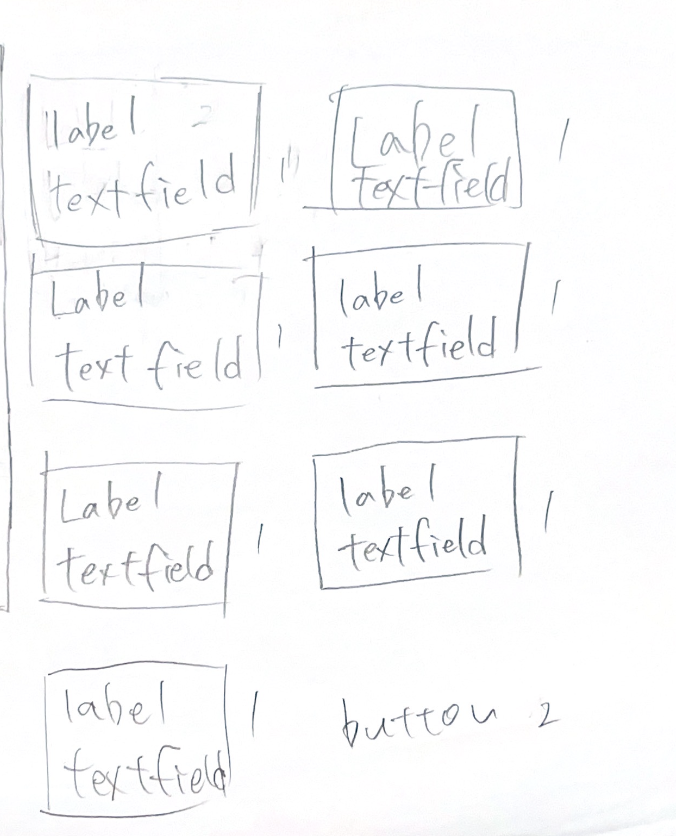
\includegraphics[width=50mm]{img/usertest_viewstructure_2.png}
    \end{center}
    \caption{被験者B記入用紙}
    \label{fig:usertest_viewstructure_2}
  \end{minipage}
\end{figure}

\begin{figure}[htbp]
  \begin{minipage}{\hsize}
    \begin{center}
       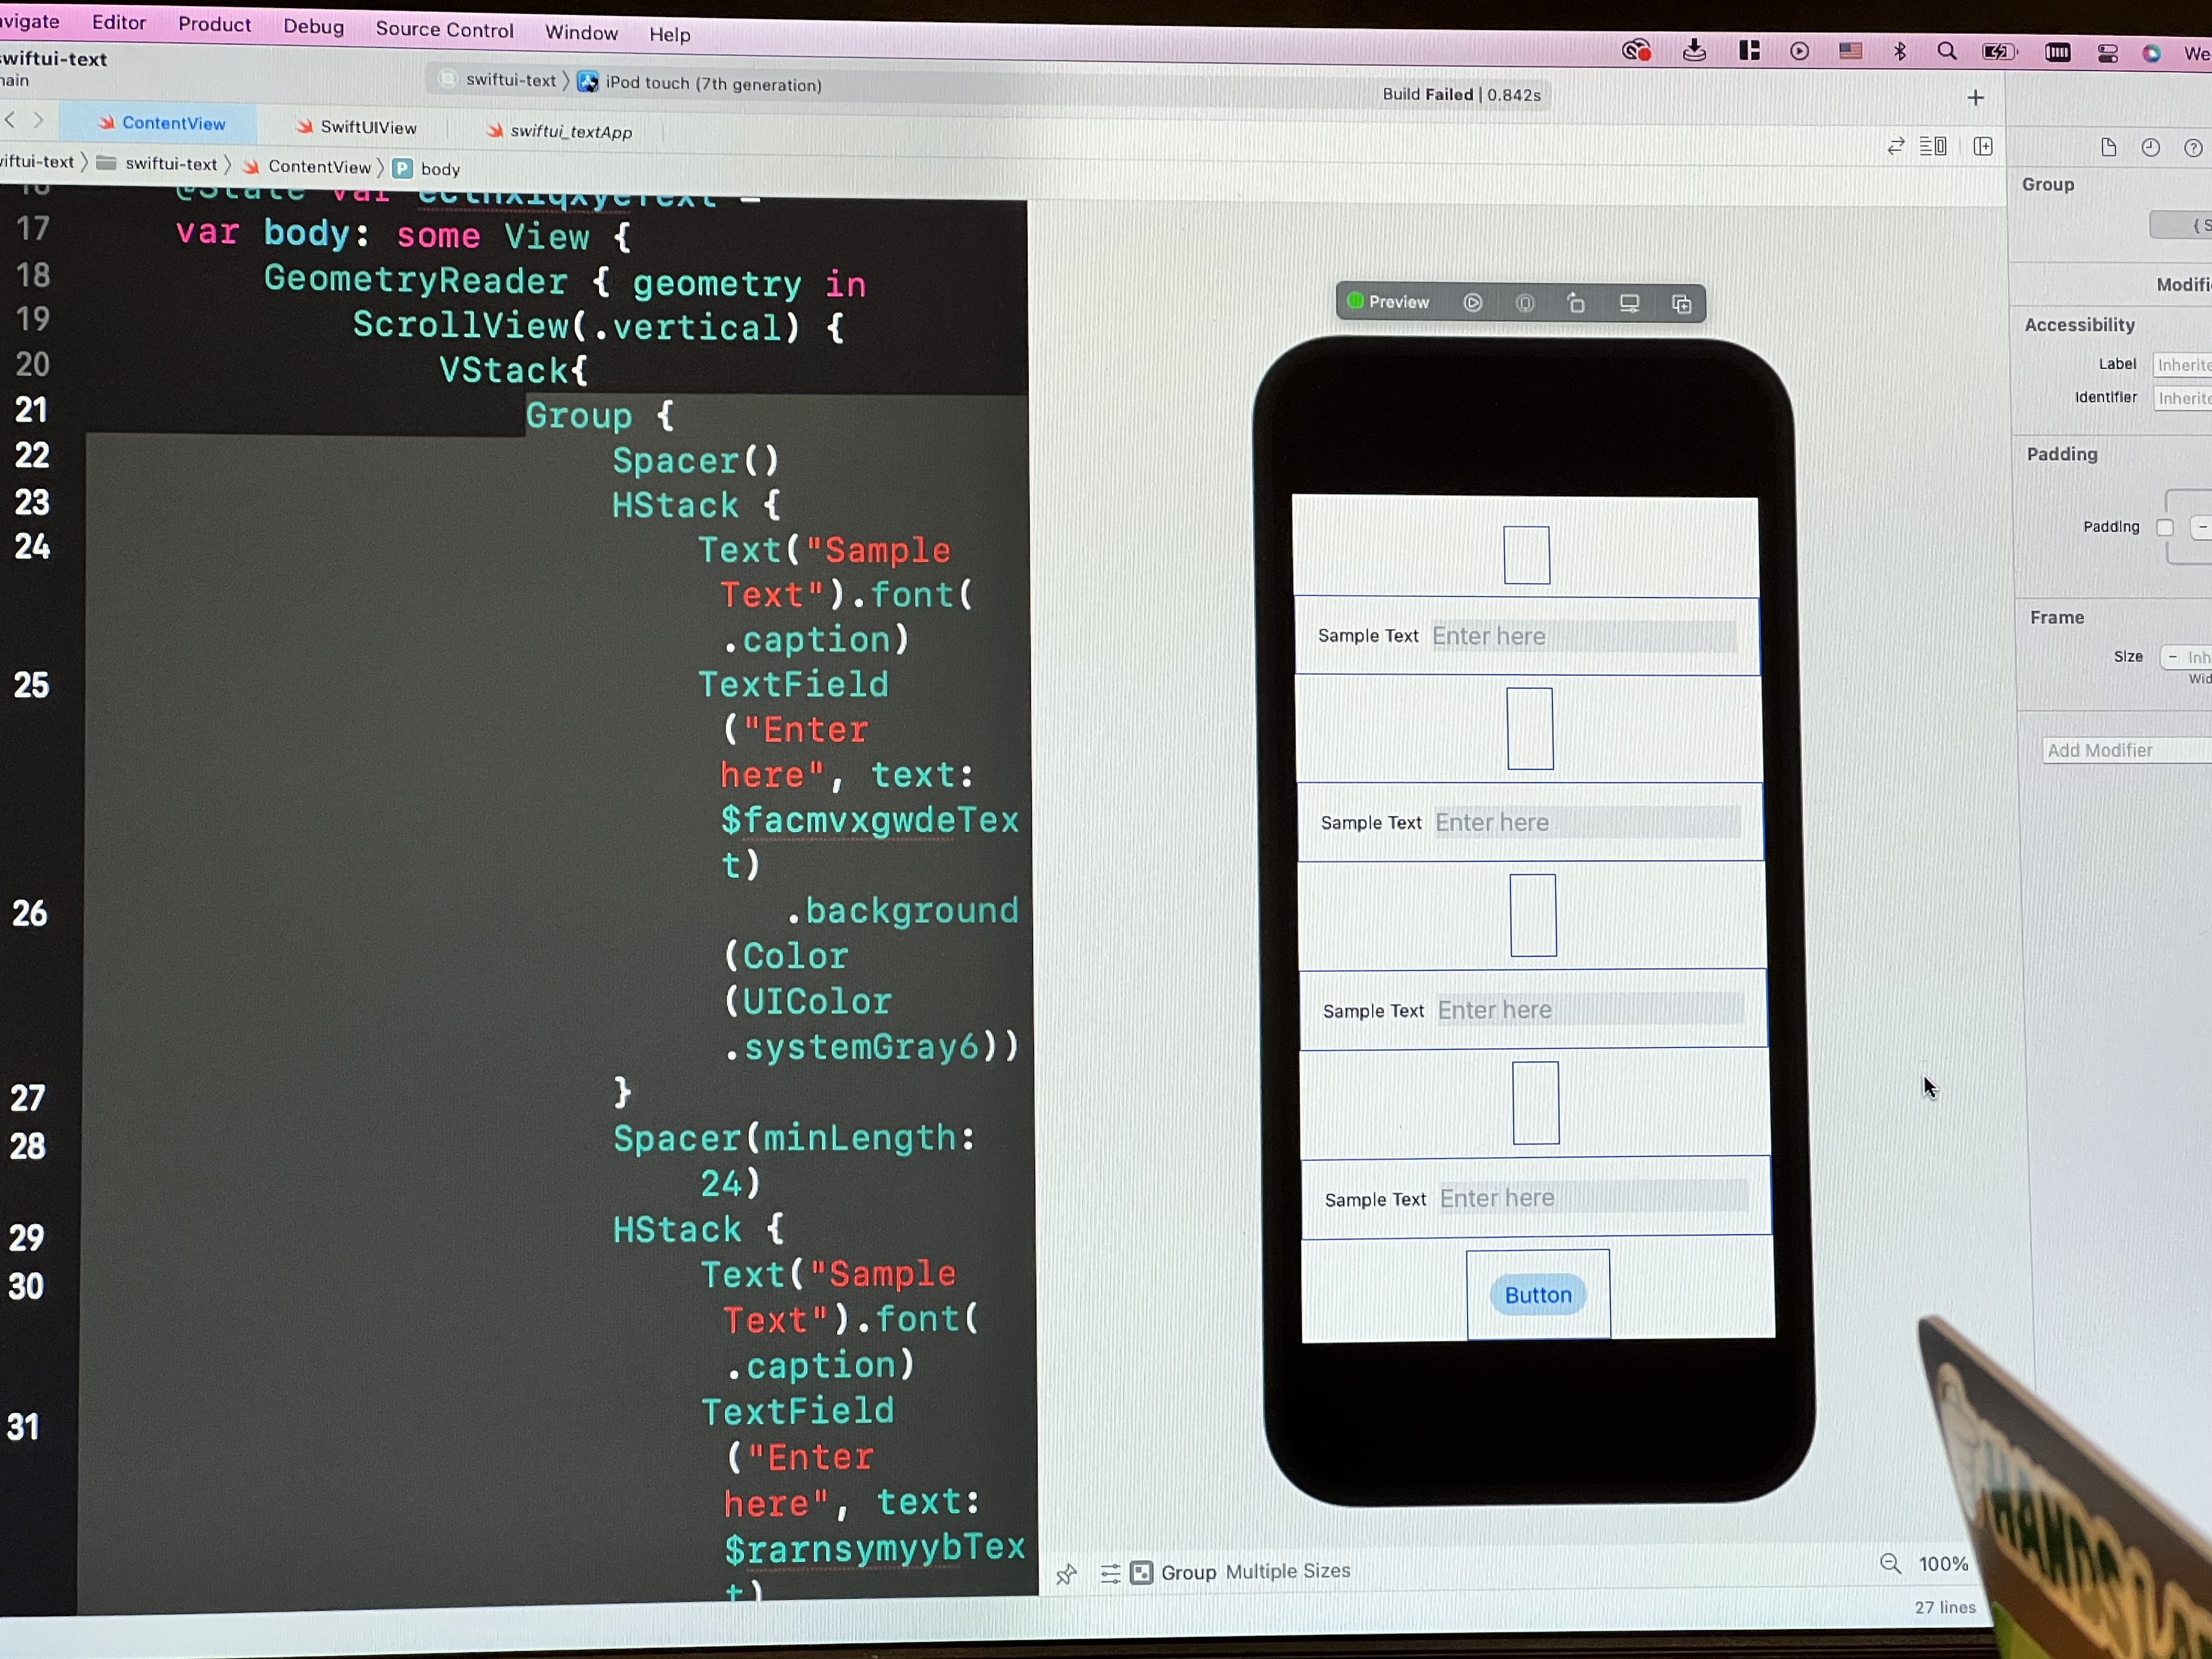
\includegraphics[width=100mm]{img/usertest_autogen_2.jpeg}
    \end{center}
    \caption{被験者B自動生成UI}
    \label{fig:usertest_autogen_2}
  \end{minipage}
\end{figure}


\begin{figure}[htbp]
  \begin{minipage}{\hsize}
    \begin{center}
       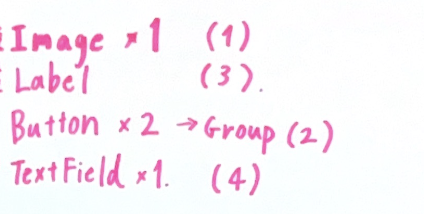
\includegraphics[width=50mm]{img/usertest_viewstructure_3.png}
    \end{center}
    \caption{被験者C記入用紙}
    \label{fig:usertest_viewstructure_3}
  \end{minipage}
\end{figure}

%\begin{figure}[htbp]
%  \begin{minipage}{\hsize}
%    \begin{center}
%       \includegraphics[width=100mm]{img/usertest_autogen_3.jpeg}
%    \end{center}
%    \caption{被験者C自動生成UI}
%    \label{fig:usertest_autogen_3}
%  \end{minipage}
%\end{figure}


\begin{figure}[htbp]
  \begin{minipage}{\hsize}
    \begin{center}
       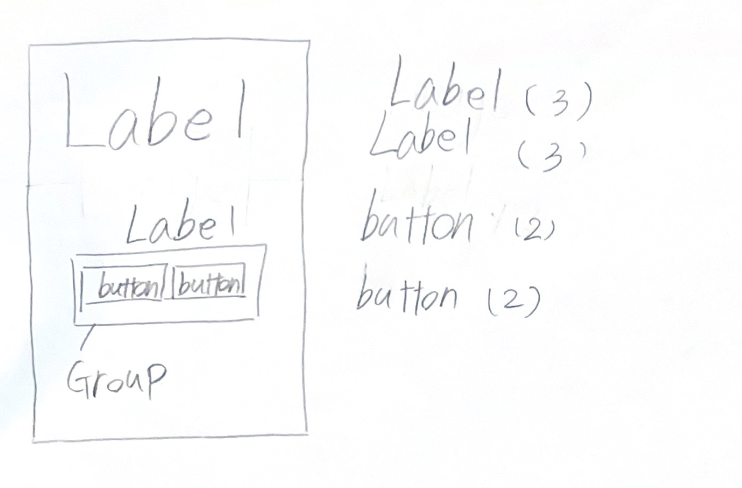
\includegraphics[width=50mm]{img/usertest_viewstructure_4.png}
    \end{center}
    \caption{被験者D記入用紙}
    \label{fig:usertest_viewstructure_4}
  \end{minipage}
\end{figure}

\begin{figure}[htbp]
  \begin{minipage}{\hsize}
    \begin{center}
       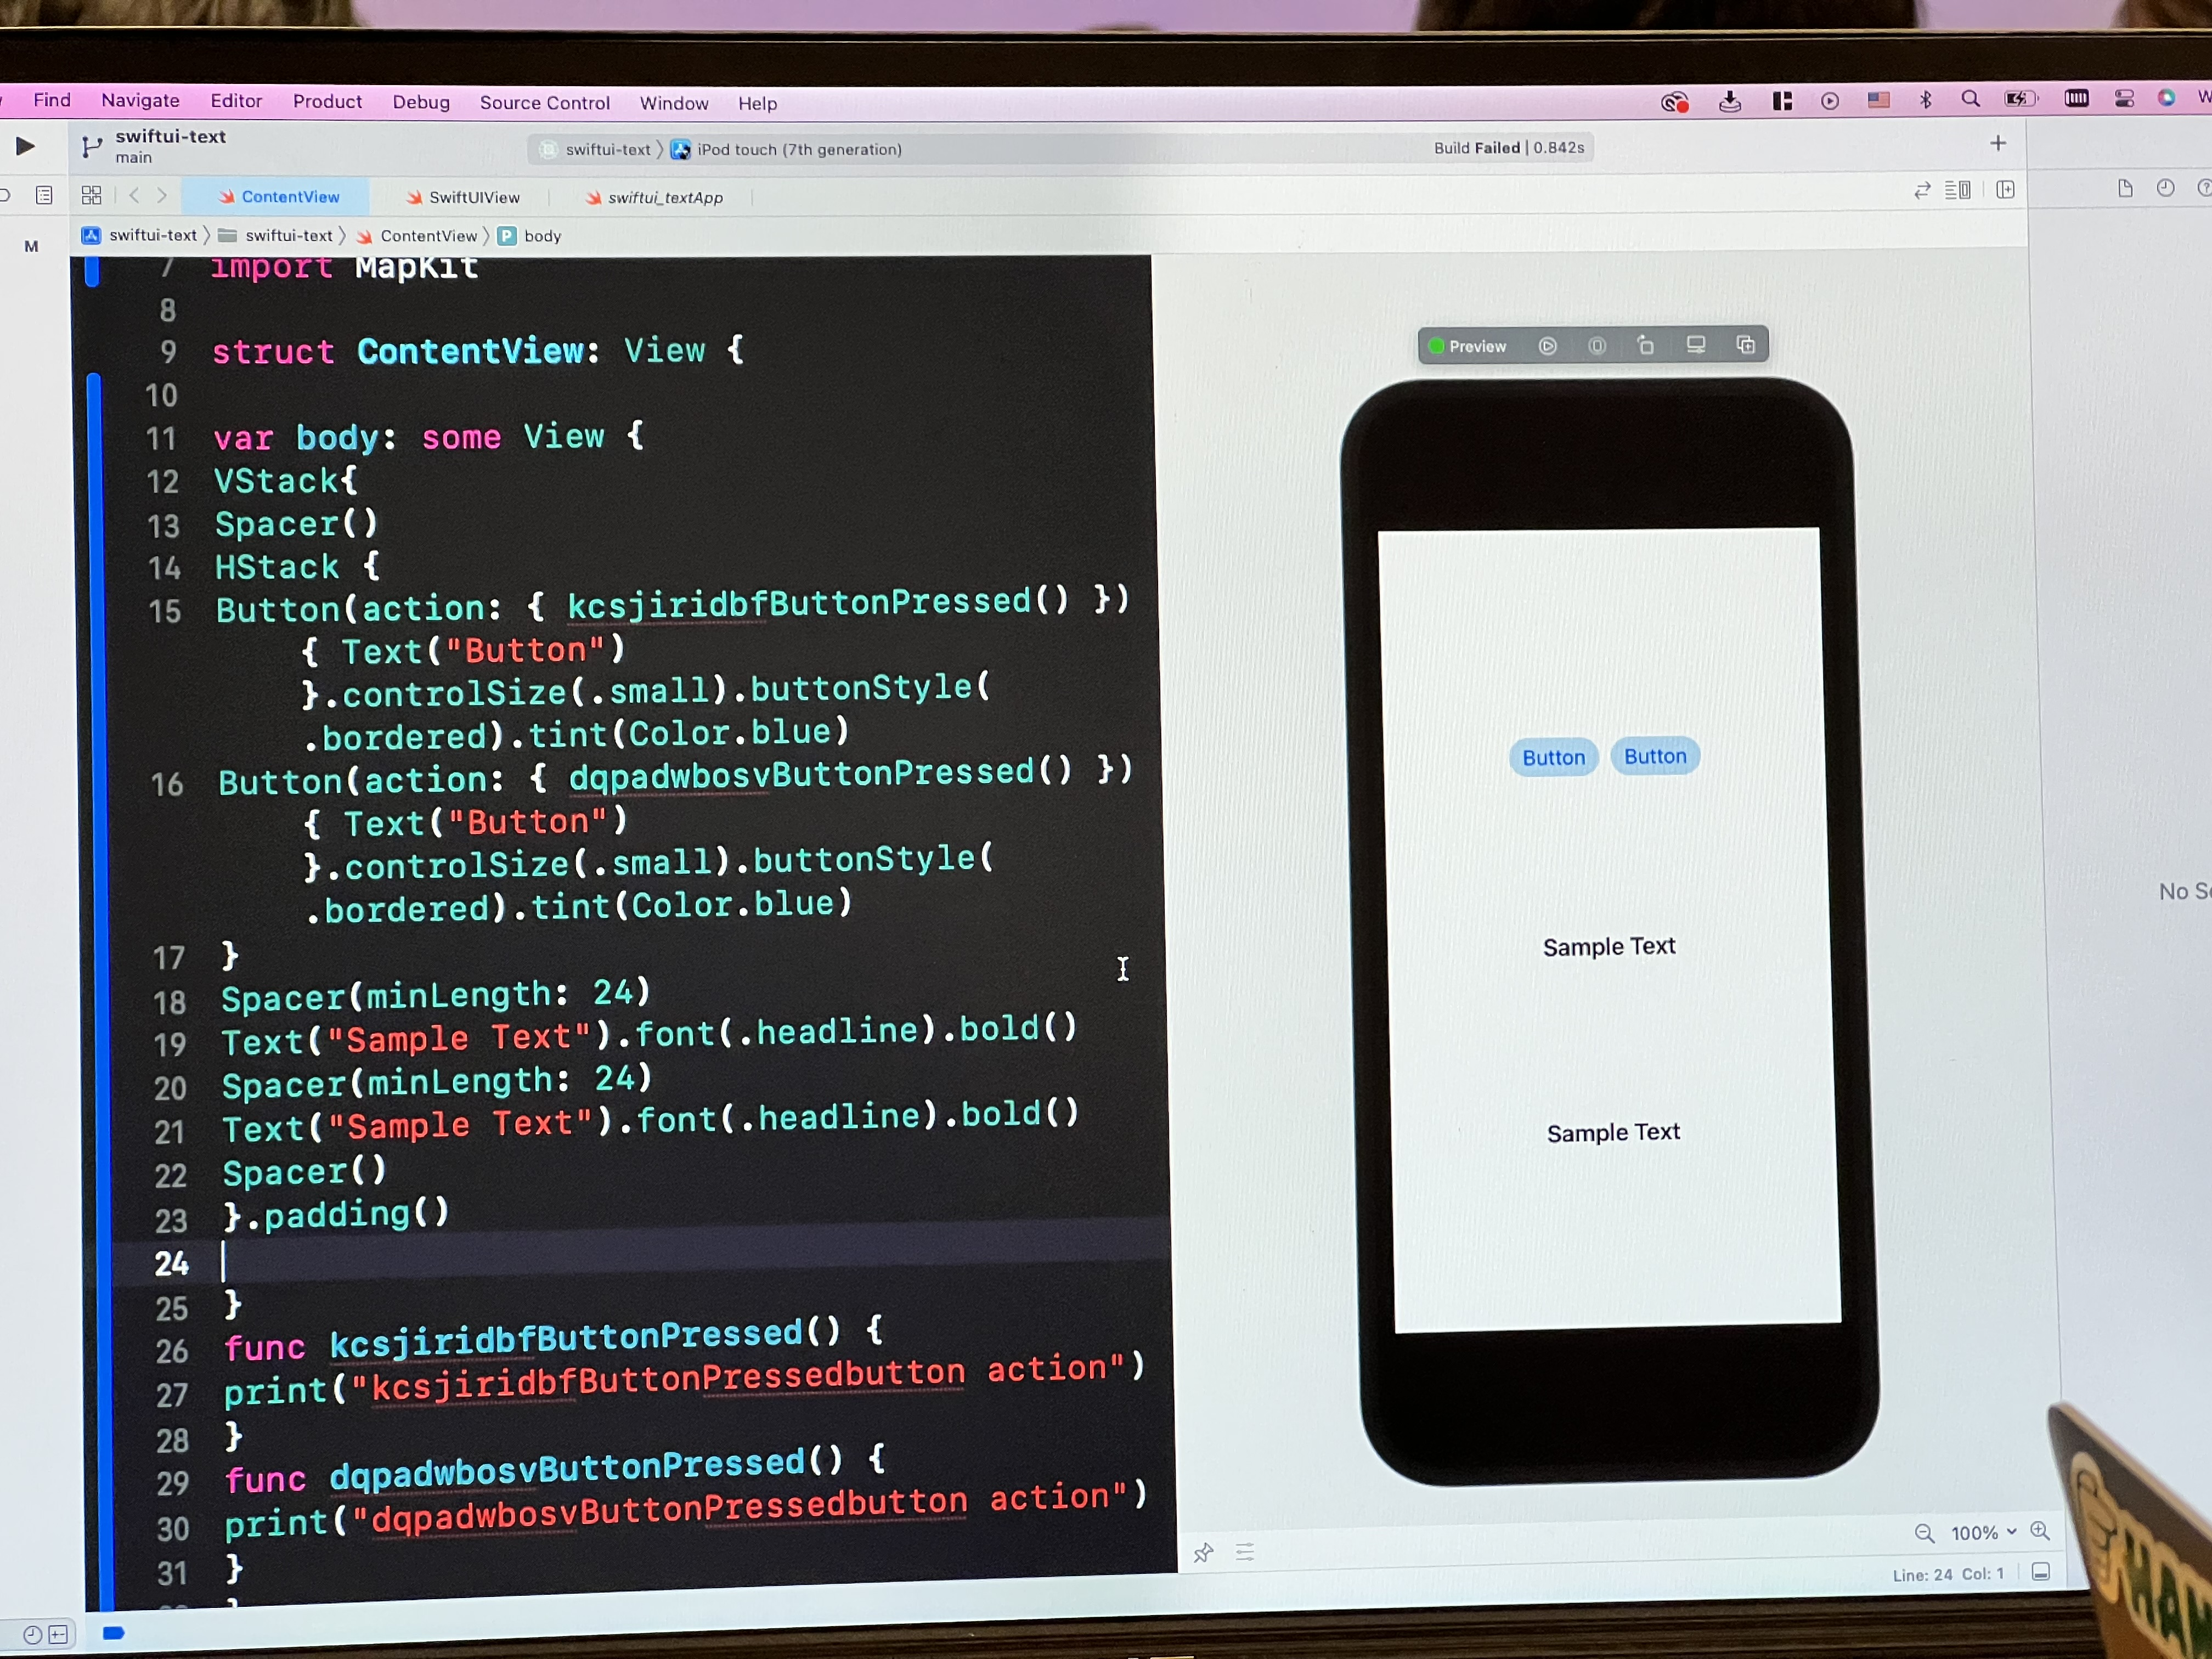
\includegraphics[width=100mm]{img/usertest_autogen_4.jpeg}
    \end{center}
    \caption{被験者D自動生成UI}
    \label{fig:usertest_autogen_4}
  \end{minipage}
\end{figure}


\begin{figure}[htbp]
  \begin{minipage}{\hsize}
    \begin{center}
       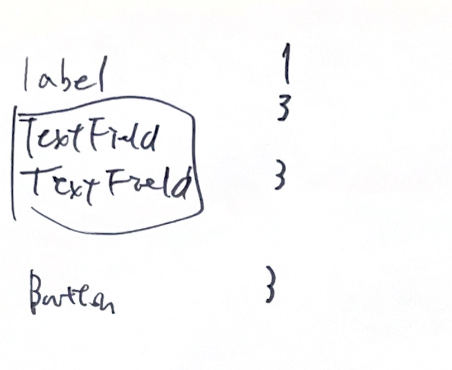
\includegraphics[width=50mm]{img/usertest_viewstructure_5.png}
    \end{center}
    \caption{被験者E記入用紙}
    \label{fig:usertest_viewstructure_5}
  \end{minipage}
\end{figure}

\begin{figure}[htbp]
  \begin{minipage}{\hsize}
    \begin{center}
       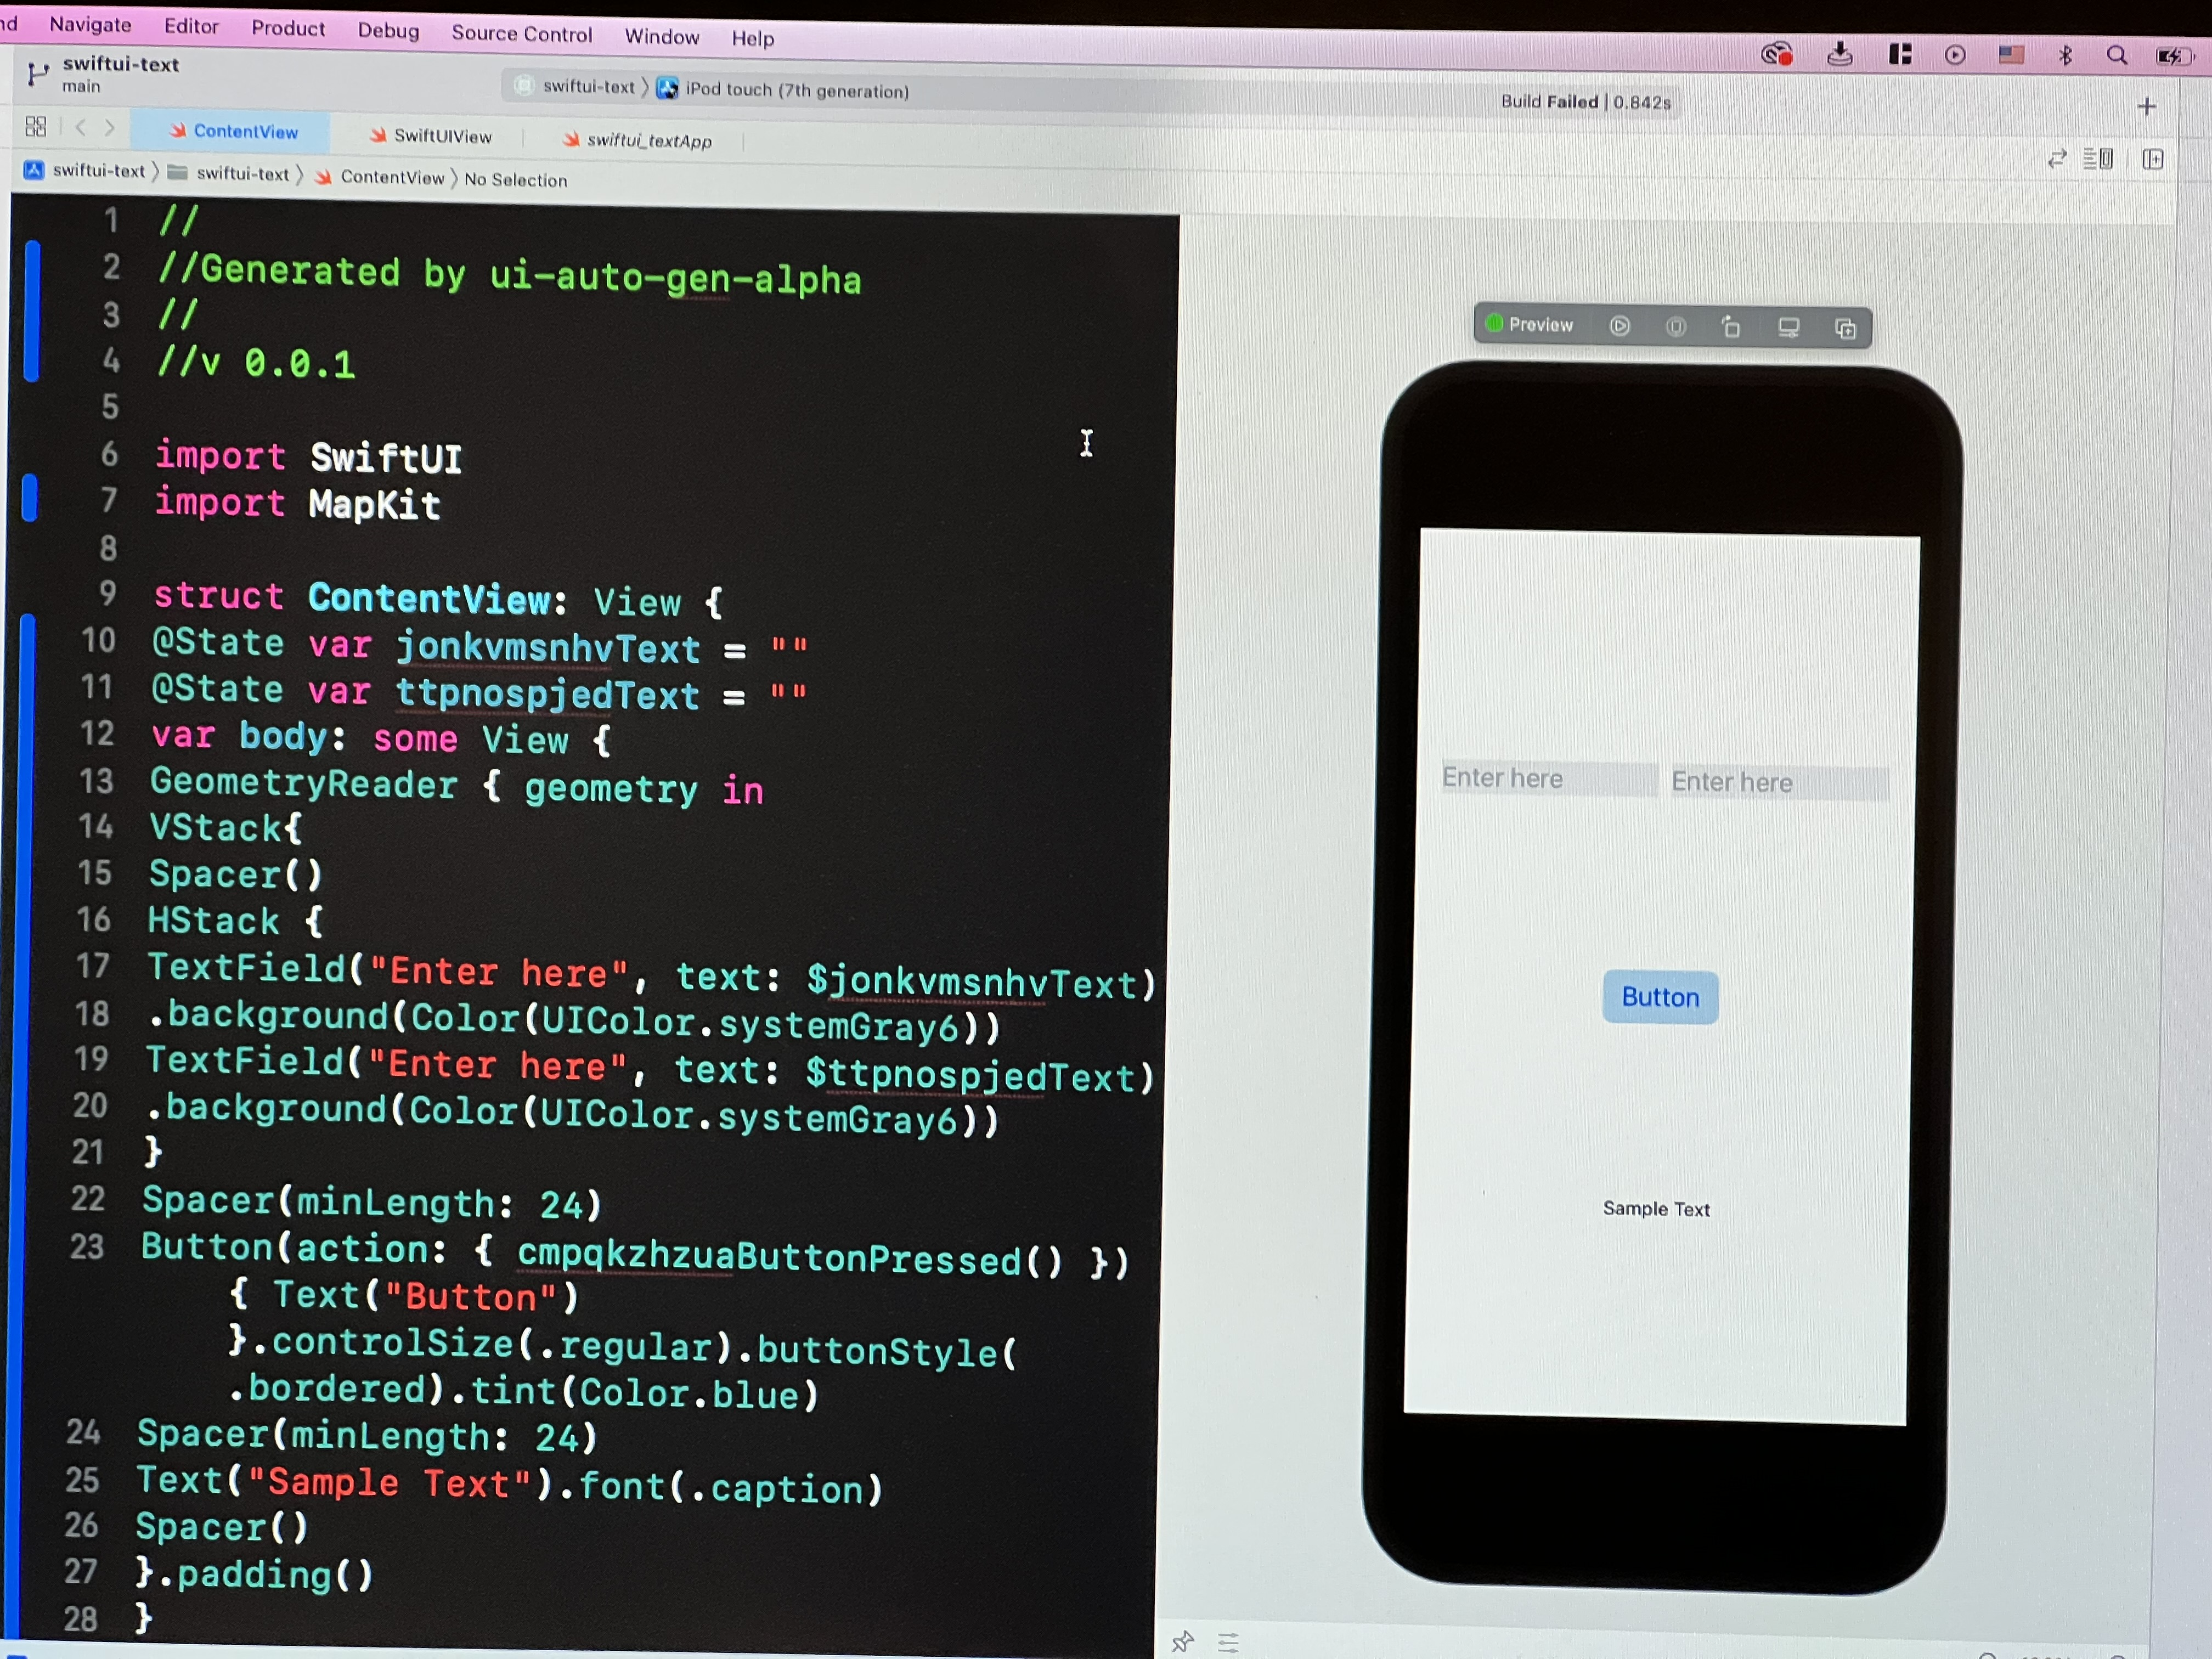
\includegraphics[width=100mm]{img/usertest_autogen_5-1.jpeg}
    \end{center}
    \caption{被験者E自動生成UI}
    \label{fig:usertest_autogen_5-1}
  \end{minipage}
\end{figure}

\begin{figure}[htbp]
  \begin{minipage}{\hsize}
    \begin{center}
       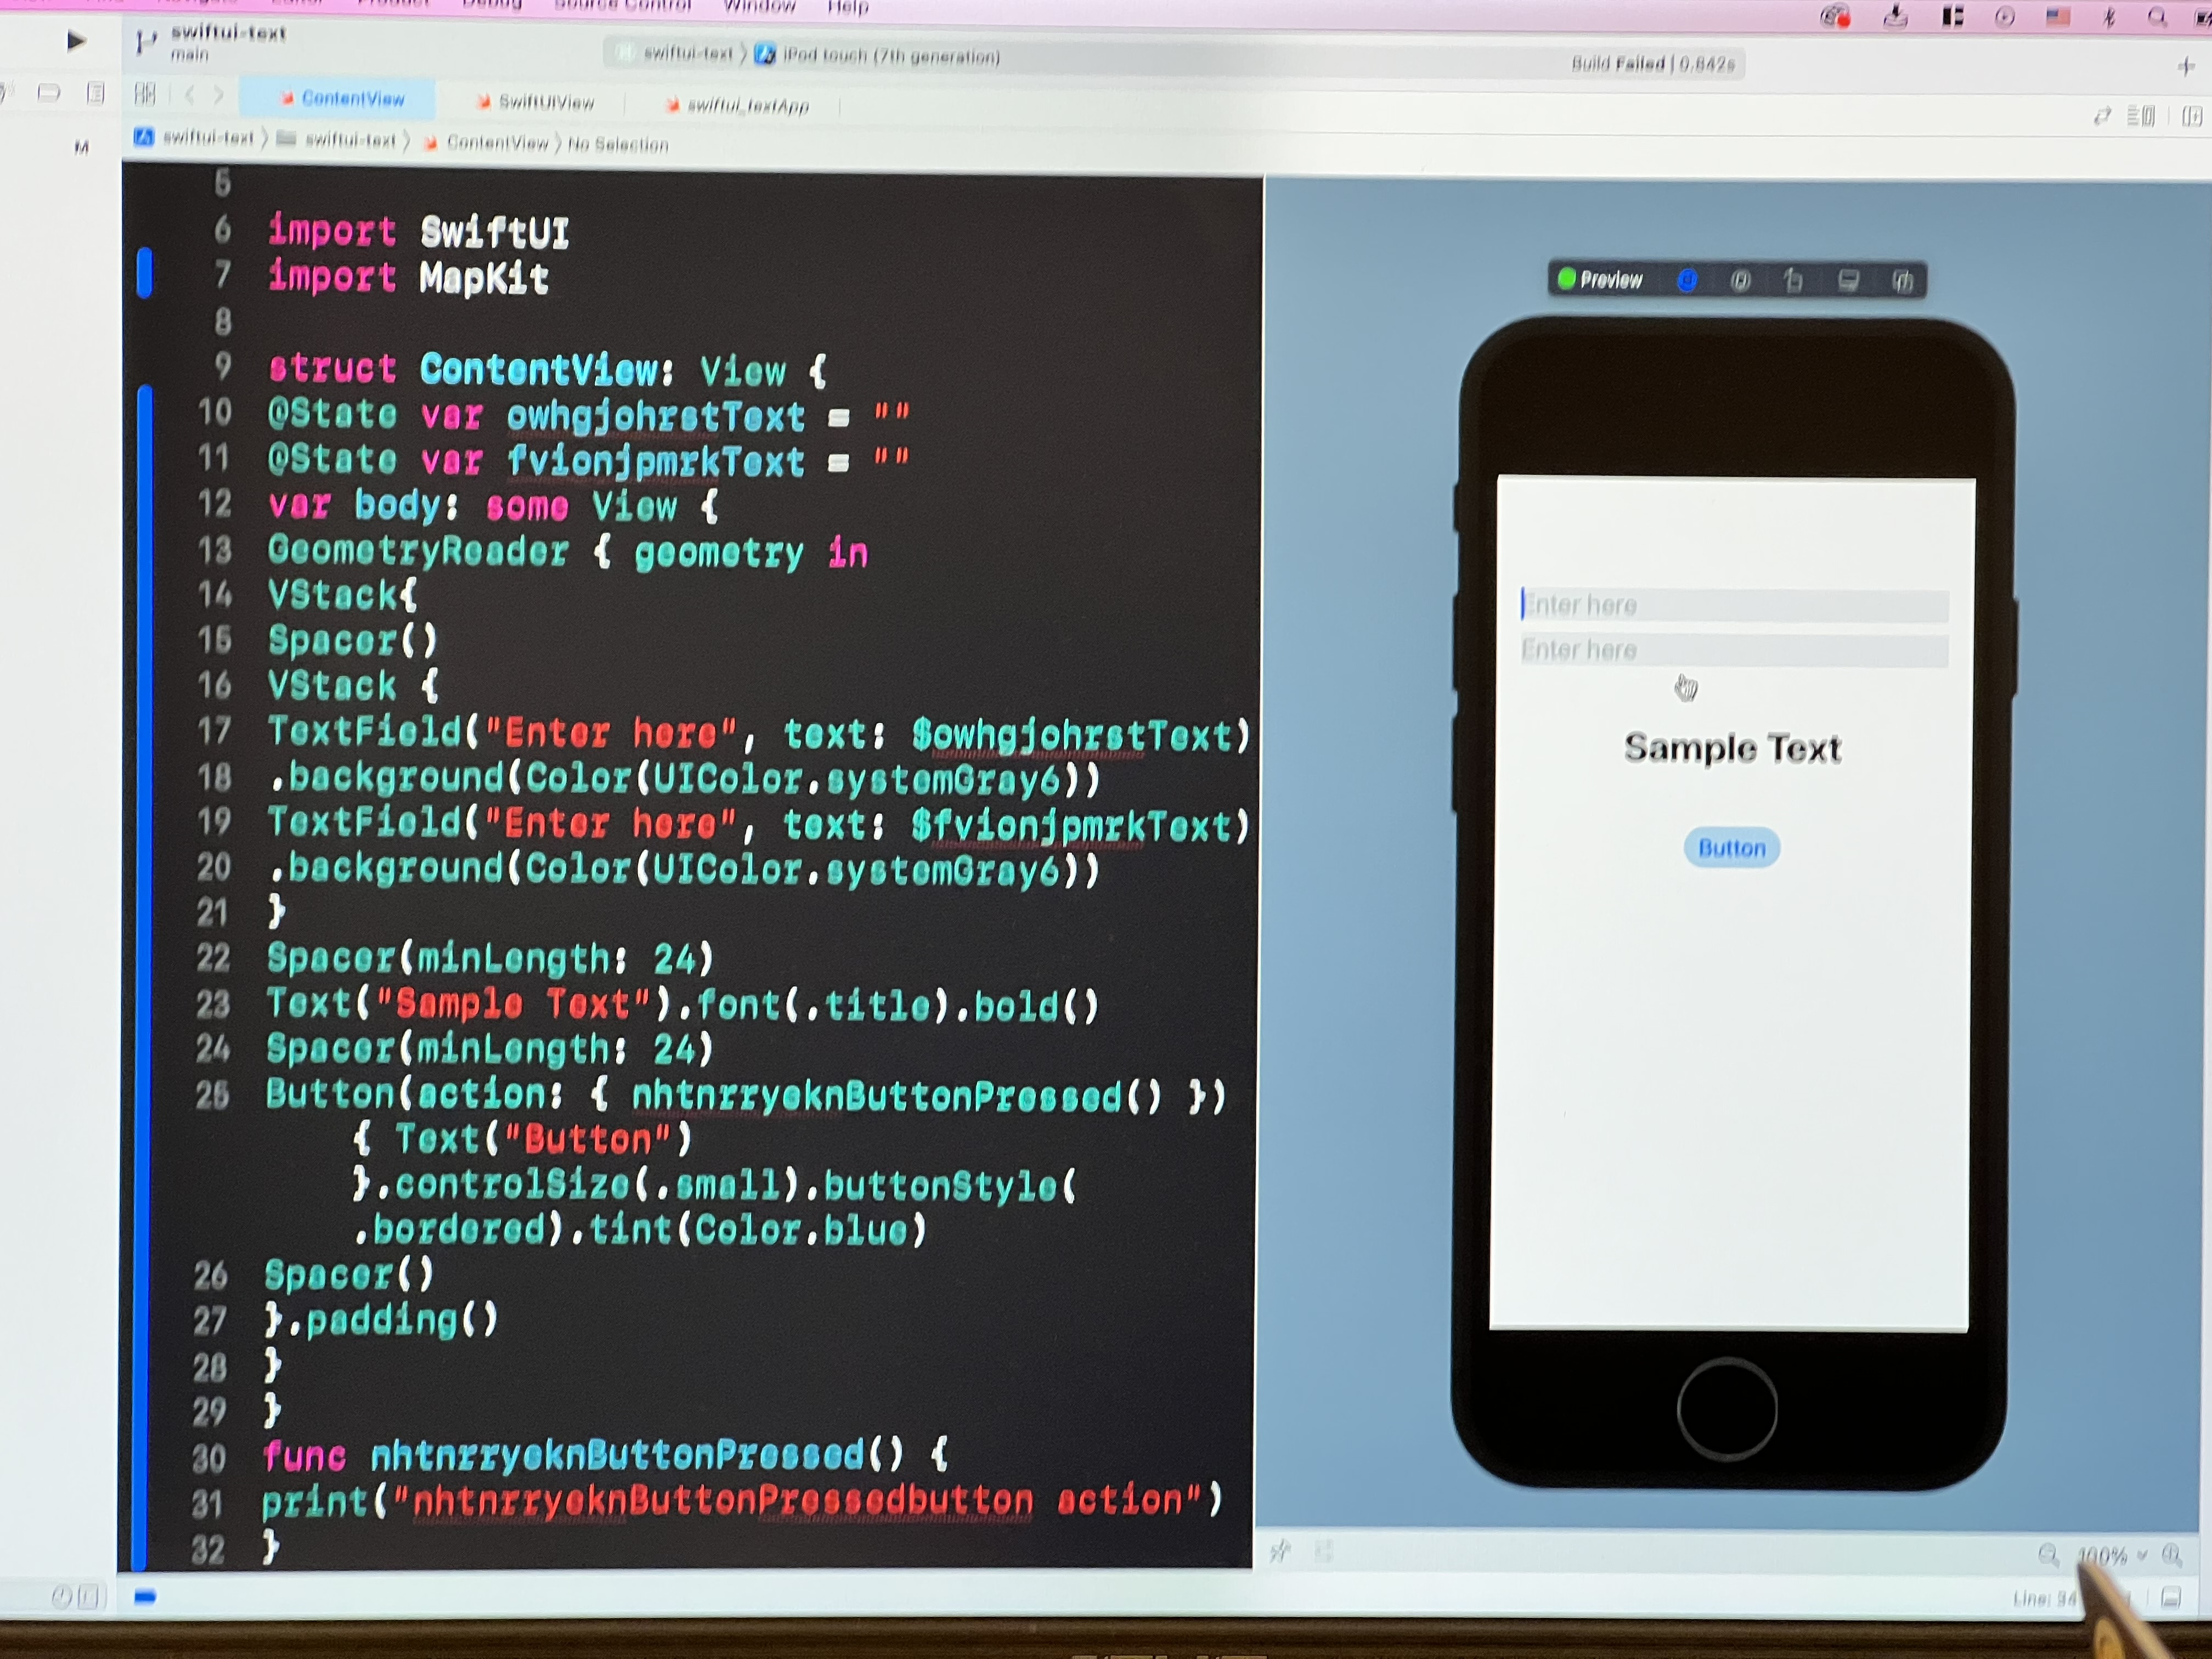
\includegraphics[width=100mm]{img/usertest_autogen_5-2.jpeg}
    \end{center}
    \caption{被験者E自動生成UI-2}
    \label{fig:usertest_autogen_5-2}
  \end{minipage}
\end{figure}



\subsection{結果と考察}
本実験を通して,既存UIを本システムで再現すること,ある程度アプリ開発について知識のある人なら本システムを利用してUIを生成することが可能であることが明らかになった.またアンケート結果によると(付録A, Bを参照)UIの生成を自動化することで効率化が図れることがわかった.

また普段デザインの見栄えを考えるあまりUIとしての本来の目的を見失いがちになるとの意見もあった.本システムはそのような場合にでも本来の目的に向かって進むことができるツールになり得る.

そしてUIの設計開発ではダークモード対応,多画面サイズ対応,アクセシビリティ対応等工数はかかるものの,単純な作業が必要である.この部分についてもアンケートで実装する上で大変だと思うことで回答されており,本自動生成システムを使用することで自動で実装されるため本システムはとても有用であるといえる.





















